\documentclass[10pt, a4paper, italian]{article}
\usepackage[T1]{fontenc}
\usepackage[utf8]{inputenc}
\usepackage{amsmath, amssymb, amsthm, thmtools, amsfonts, mathtools}
\usepackage{nicefrac}
\usepackage{calc}
\usepackage[pdftex, hyperindex, plainpages=false]{hyperref}
\usepackage[nameinlink]{cleveref} %load before classicthesis (clash)
%\usepackage[nochapters,pdfspacing]{classicthesis}
\usepackage{siunitx}
\usepackage[siunitx]{circuitikz}

\usepackage[a4paper]{geometry}
\usepackage{float}
\usepackage{mdframed}
\usepackage{titling}
\usepackage{booktabs}
\usepackage{graphicx}
\usepackage{caption, subcaption}
\usepackage{xcolor}
\usepackage[italian]{babel}
\usepackage{pgfplots}
\usepackage{listings}
%\usepackage{lmodern}
\usepackage{url}
\usepackage{enumitem}
\usepackage{tikz} %loads after classicthesis (xcolor incompat)

% lets graphicx know path where figures to be included are found
\graphicspath{{../figs/}}
\makeatletter
\def\input@path{{../figs/}}
%or: \def\input@path{{/path/to/folder/}{/path/to/other/folder/}}
\makeatother

% tikz pgf plots setup
\usepgfplotslibrary{external}
\pgfplotsset{compat=1.15}
%\tikzexternalize

% spaces and significant digits/figures for measurements
\sisetup{free-standing-units, space-before-unit, number-unit-product = \;,
scientific-notation = false, round-mode = figures, round-precision = 1,}

% turns all (hyperlinked) references black [default is blue]
\hypersetup{
	linktoc=all,
	colorlinks=true,
	linkcolor=black
}

% code listings config
%\lstset{
%language=Python,
%basicstyle=\ttfamily,
%columns=fullflexible,
%keepspaces=true,
%}

% mdframed (for boxed text) configuration
\mdfsetup{linewidth=0.6pt}

% Default fixed font does not support bold face
\DeclareFixedFont{\ttb}{T1}{txtt}{bx}{n}{12} % for bold
\DeclareFixedFont{\ttm}{T1}{txtt}{m}{n}{12}  % for normal

% Custom colors
\usepackage{color}
\definecolor{deepblue}{rgb}{0,0,0.5}
\definecolor{deepred}{rgb}{0.6,0,0}
\definecolor{deepgreen}{rgb}{0,0.5,0}

% Commands 
\newcommand{\executeiffilenewer}[3]{%
	\ifnum\pdfstrcmp{\pdffilemoddate{#1}}%
		{\pdffilemoddate{#2}}>0%
	{\immediate\write18{#3}}\fi%
}
% input .svg --> .pdf_tex graphs
%\newcommand{\includesvg}[1]{%
%	\executeiffilenewer{#1.svg}{#1.pdf}%
%	{inkscape -z -D --file=#1.svg %
%	--export-pdf=#1.pdf --export-latex}%
%	\input{#1.pdf_tex}%
%}
% Thanks UniPi's Department of Physics E. Fermi
\newcommand{\thanksdf}{(\thanks{Dipartimento di Fisica E.~Fermi,%
Universit\`a di Pisa - Pisa, Italy.}\;)}

% hyperlink to email address
\newcommand{\mail}[1]{\href{mailto:#1}{\textsf{#1}}}

% \vec for bold vectors, instead of overarrows (now "\arrvec")
\let\arrvec=\vec
\renewcommand{\vec}[1]{\boldsymbol #1}
% replaces straight phi with slanted phi
\renewcommand{\phi}{\varphi}
% replaces straight eps with curved epsilon
\newcommand{\eps}{\varepsilon}
% abbreviation for (sub_/super^)scripts of \lim, \sum,... in inline math
\newcommand{\ds}{\displaystyle}

% blackboard/number set letters
\newcommand{\CC}{\mathbb C}
\newcommand{\HH}{\mathbb H}
\newcommand{\KK}{\mathbb K}
\newcommand{\NN}{\mathbb N}
\newcommand{\PP}{\mathbb P}
\newcommand{\QQ}{\mathbb Q}
\newcommand{\RR}{\mathbb R}
\newcommand{\ZZ}{\mathbb Z}

\newcommand{\Abs}[1]{{\left\Vert #1\right\Vert}}
\newcommand{\enclose}[1]{{\left( #1 \right)}}
\newcommand{\Enclose}[1]{{\left[ #1 \right]}}
\newcommand{\floor}[1]{\left\lfloor #1 \right\rfloor}
\newcommand{\ceil}[1]{\left\lceil #1 \right\rceil}
\newcommand{\To}{\rightrightarrows}

% Math operators
\DeclareMathOperator{\divergence}{div}
\renewcommand{\div}{\divergence}
\DeclareMathOperator{\Imaginarypart}{Im}
\renewcommand{\Im}{\Imaginarypart}
\DeclareMathOperator{\Realpart}{Re}
\renewcommand{\Re}{\Realpart}
%\DeclareMathOperator{\arg}{arg}
\DeclareMathOperator{\tg}{tg}
\DeclareMathOperator{\arctg}{arctg}
\DeclareMathOperator{\settsinh}{settsinh}
\DeclareMathOperator{\settcosh}{settcosh}
\DeclareMathOperator{\tr}{tr}
\DeclareMathOperator{\im}{im}
\DeclareMathOperator{\sgn}{sgn}
\DeclareMathOperator{\diag}{diag}

\DeclarePairedDelimiter{\norm}{\lVert}{\rVert}
\DeclarePairedDelimiter{\scalar}{\langle}{\rangle}

% Logarithm with arbitrary base.
% -> log_10
\newcommand{\llog}[1][10]{\log_{#1}}

% Absolute value.
% -> |x|
\newcommand{\abs}[1]{\left| #1 \right|}

% Powers.
% -> x^a
\newcommand{\power}[2][2]{\left( #2 \right)^{#1}}

% Square.
% -> x^2
\newcommand{\sq}[1]{\power[2]{#1}}

% Expansion of the binomial coefficient.
% -> n1!/(n2!(n1 - n2)!)
\newcommand{\binomexpr}[2]{\frac{#1!}{#2!(#1 - #2)!}}

% Expression evaluation at a given point with square brackets.
% -> [x]_{a}
\newcommand{\at}[2]{\left[ #1\right]_{\makebox[-1pt][l]{${\scriptstyle#2}$}}}

% Expression evaluation in an interval.
% -> [x] _{a}^{b}
\newcommand{\eval}[3]{\left.#1%
  \right|_{\makebox[-1pt][l]{${\scriptstyle#2}$}}^{\makebox[-1pt][l]{${\scriptstyle#3}$}}}

% Upright d in math mode (for differentials).
% -> d
\newcommand{\ud}{\mathrm{d}}

% Differential.
% -> dx
\newcommand{\diff}[1][x]{\,\ud{#1}}

% Base command for defining derivatives.
% -> df/dx or d^kf/dx^k
\newcommand{\basederivative}[4][]{%
  \displaystyle%
  \ifx\\#1\\\frac{#4#2}{#4#3}%
  \else%
  \frac{#4^#1#2}{#4#3^#1}%
  \fi%
}

% Total derivative.
% -> df/dx(x) or d^kf/dx^k(x)
\newcommand{\td}[4][]{%
  \basederivative[#1]{#2}{#3}{\ud}%
  \ifx\\#4\\%
  \else%
  \mkern-4mu\left(#4\right)%
  \fi%
}

% Partial derivative.
% -> df/dx(x) or d^kf/dx^k(x)
\newcommand{\pd}[4][]{%
  \basederivative[#1]{#2}{#3}{\partial}%
  \ifx\\#4\\%
  \else%
  \mkern-4mu\left(#4\right)%
  \fi%
}

\newcommand{\intinf}{\int_{-\infty}^{\infty}\!\!\!}

\newcommand{\cinterval}[2]{\left[\, #1,~#2 \,\right]}

\newcommand{\linterval}[2]{\left[\, #1,~#2 \,\right)}

\newcommand{\rinterval}[2]{\left(\, #1,~#2 \,\right]}

\newcommand{\ointerval}[2]{\left(\, #1,~#2 \,\right)}

\newcommand{\prob}[1]{\displaystyle P\left(#1\right)}

\newcommand{\pvalue}{\emph{$p$-value}}

\newcommand{\cond}{\,|\,}

\newcommand{\expect}[1]{\displaystyle E\left[#1\right]}

\newcommand{\mom}[2][]{\displaystyle {\cal M}_{#2}\ifx\\#1\\\else(#1)\fi}

\newcommand{\momalg}[1]{\displaystyle \lambda_{#1}}

\newcommand{\momcen}[1]{\displaystyle \mu_{#1}}

\newcommand{\skewness}{\displaystyle \gamma_1}

\newcommand{\kurtosis}{\displaystyle \gamma_2}

\newcommand{\charf}[1][x]{\phi_{#1}}

\newcommand{\momgenf}[1][x]{M_{#1}}

\newcommand{\fwhm}{{\scriptstyle \textsc{FWHM}}}

\newcommand{\hwhm}{{\scriptstyle \textsc{HWHM}}}

\newcommand{\median}{\mu_{\nicefrac{1}{2}}}

\newcommand{\var}[1]{\ensuremath{\text{Var}\left(#1\right)}}

\newcommand{\cov}[2]{\ensuremath{\text{Cov}\left(#1, #2\right)}}

\newcommand{\corr}[2]{\ensuremath{\text{Corr}\left(#1, #2\right)}}

\newcommand{\like}{\mathcal L}

\newcommand{\likelihood}[2][]{\like\ifx\\#2\\\else(#2\ifx\\#1\\\else;#1\fi)\fi}

\newcommand{\chisq}{\ensuremath{\chi^2}}

\newcommand{\chisquare}[2][]{\chisq\ifx\\#2\\\else(#2\ifx\\#1\\\else;#1\fi)\fi}

\newcommand{\loglikelihood}[2][]{\log\likelihood[#1]{#2}}

\newcommand{\pdf}[3][]{#2(#3\ifx\\#1\\\else;#1\fi)}

\newcommand{\binomialpdf}[2][]{\pdf[#1]{\mathcal B}{#2}}

\newcommand{\multinomialpdf}[2][]{\pdf[#1]{\mathcal M}{#2}}

\newcommand{\poissonpdf}[2][]{\pdf[#1]{\mathcal P}{#2}}

\newcommand{\uniformpdf}[2][]{\pdf[#1]{u}{#2}}

\newcommand{\exponentialpdf}[2][]{\pdf[#1]{\varepsilon}{#2}}

\newcommand{\gausspdf}[2][]{\pdf[#1]{N}{#2}}

\newcommand{\chisquarepdf}[2][]{\pdf[#1]{\wp}{#2}}

\newcommand{\cauchypdf}[2][]{\pdf[#1]{c}{#2}}

\newcommand{\erf}[1]{\ensuremath{\text{erf}\left(#1\right)}}

\newcommand{\dccases}[4][]{#2 \ifx\\#2\\\else=\fi %
  \begin{cases}
    \displaystyle #3 & \text{per variabili discrete}\\
    \displaystyle #4 & \text{per variabili continue}#1
  \end{cases}
}
% sub/super-scriptable for all symbol as math operator 
\newcommand\Scaleforall[1]{\vcenter{\hbox{\scalefont{#1}$\forall$}}}

\DeclareMathOperator*\forevery{%
  \vphantom\sum
  \mathchoice{\Scaleforall{2}}{\Scaleforall{1.4}}{\Scaleforall{1}}{\Scaleforall{0.75}}}
\geometry{left=2cm, right=2cm, top=2cm, bottom=2cm}

% indexes subsections with letters, sections with numbers (1.a, 1.b, ...)
\renewcommand{\thesubsection}{\thesection.\alph{subsection}}

% lets graphicx know path where figures to be included are found
\graphicspath{{../figs/}}

\author{Gruppo 1.AC \\ Bernardo Tomelleri}
\title{Es06A: Oscillatore sinusoidale a ponte di Wien con OpAmp}
\begin{document}
\date{\today}
\maketitle

\setcounter{section}{0}

\section*{Misura componenti dei circuiti}
\begin{table}[htbp]
\centering
\begin{tabular}{cccccc}
\toprule
Resistenze $[\si{k\ohm}]$ & $R$ & $\sigma R$ & Capacità $[\si{n\F}]$ & $C$ &
$\sigma C$ \\
\midrule
\midrule
$R_1$	  & 9.91	& 0.08	 & $C_1$ & 10.0		 & 0.4 \\
$R_2$	  & 9.91	& 0.08 	 & $C_2$ & 10.0		 & 0.4 \\
$R_3$	  & 9.93	& 0.08	 & & & \\
$R_4$	  & 9.93	& 0.08	 & & & \\
$R_5$	  & 9.95	& 0.08	 & & & \\
$R$		  & 9.49	& 0.08	 & & & \\
\bottomrule     
\end{tabular}
\caption{Valori di resistenza e capacità misurate per i componenti dei
circuiti studiati. \label{tab: rcmes}}
\end{table}

Riportiamo per completezza anche i valori delle tensioni di alimentazione
continue per l'op-amp misurate con il multimetro
\begin{align*}
V_{CC} &= 4.99 \pm 0.03 \si{\V} \\
V_{EE} &= -4.99 \pm 0.03 \si{\V}
\end{align*}

Per tutto il resto della trattazione come ampiezze dei segnali si intendono
misurate non ``picco - picco'', a meno che non venga esplicitato altrimenti.

\subsection*{Nota sul metodo di fit}
Per determinare i parametri ottimali e le rispettive covarianze si \`e
implementato in \verb+Python+ un algoritmo di fit basato sui minimi quadrati
mediante la funzione \emph{curve\_fit} della libreria \texttt{SciPy}.

%=======================
\section{Apparato di misura del guadagno ad anello chiuso}
Si è montato il circuito per la misura del loop-gain
$\bar{L}(j\omega) = \beta(j\omega) \bar{A}$ nel nostro generatore di
onde sinusoidali come quello proposto nello schema in \cref{fig: aloopschm}

\begin{figure}[htbp]
    \centering
	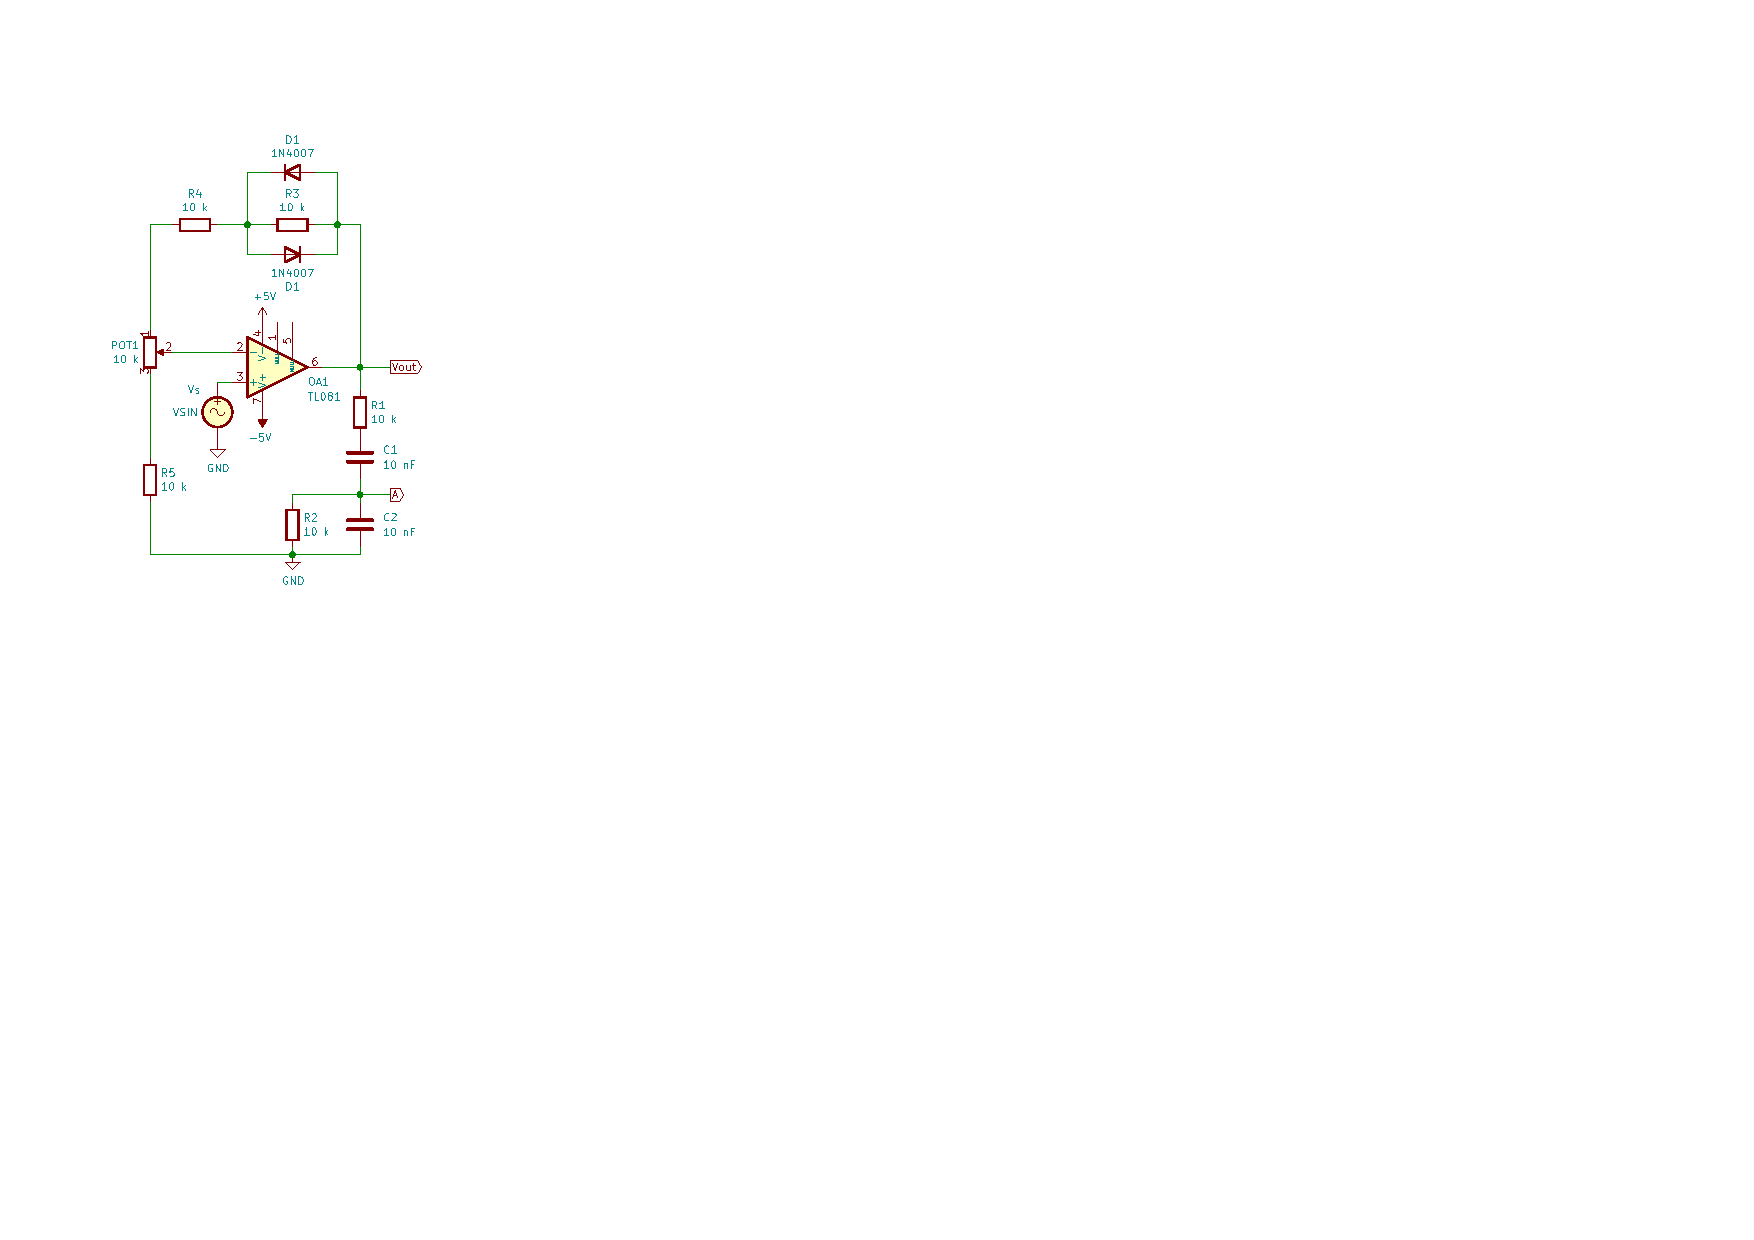
\includegraphics[scale=1.2]{aloopschm}
    \caption{Schema circuitale dell'amplificatore di carica costruito.
    \label{fig: aloopschm}}
\end{figure}

Il circuito è formato da un amplificatore non-invertente con guadagno
indipendente dalla frequenza (trascurando la presenza e risposta non lineare
dei diodi in parallelo a $R_3$ - che consideriamo dei circuiti aperti - dal
momento che supponiamo di lavorare con $V\ped{out} \sim V_{R_3}$ vincolato ad
essere in modulo minore rispetto alla tensione caratteristica del regime di
conduzione in cui questi svolgono un ruolo $V_\gamma \sim \SI{0.7}{\V}$)
\begin{equation}\label{eq: A}
A  = 1 + \frac{(1 - p)R + R_3 + R_4}{pR + R_5}
\end{equation}
in cui il parametro $p \in [0,1]$ è stato introdotto per indicare la posizione
del contatto strisciante in POT1, o meglio la frazione di resistenza
totale $R$ del potenziometro ideale che si trova tra il terminale centrale e
la resistenza $R_5$ (dunque massa). Quindi, per costruzione, quando $p = 0$
il trimmer del potenziometro è girato tutto verso il basso ($R_5$), mentre per
$p = 1$ è rivolto verso l'alto ($R_4$).

A questo si aggiunge un anello di feedback ``positivo'' il cui guadagno è dato
dal rapporto di partizione
\begin{equation} \label{eq:loop-gain-beta}
\beta(s) = \frac{Z_P}{Z_S + Z_P} = \frac{1}{Z_S/Z_P + 1}
\end{equation}
tra un'impedenza serie RC $Z_S$ e un'impedenza ``parallelo'' $Z_P$, ovverosia
\begin{align*}
Z_S &= R_1 + \frac{1}{s C_1} = R_1 \frac{s + \omega_1}{s} \\
Z_P &= \frac{R_2}{1 + s R_2 C_2} = R_2 \frac{\omega_2}{s + \omega_2}
\end{align*}
dove abbiamo indicato $\omega_1 = 1/(R_1 C_1)$ e con $\omega_2 = 1/(R_2 C_2)$.
Espandendo in termini delle singole resistenze e pulsazioni possiamo riscrivere
il fattore di feedback
\begin{equation}
\beta(s) = \frac{1}{1 + Z_S/Z_P} =
\frac{1}{1 + \frac{R_1}{R_2} \frac{(s + \omega_1)(s + \omega_2)}{s \omega_2}} =
\frac{R_2}{R_1} \frac{s \omega_2}{\omega_1 \omega_2 + s^2 +
\left[\omega_{1} + \omega_{2} \left(1 + \frac{R_2}{R_{1}}\right)\right] s}
\end{equation}
Per la condizione di Barkhausen consideriamo solo valori puramente immaginari
di $s = j\omega$, per cui troviamo
\begin{equation}
\beta(j\omega) = \frac{R_2}{R_1} \frac{j \omega \omega_2}
{\omega_1 \omega_2 - \omega^2 + j \omega
\left[\omega_1 + \omega_2 \left(1 + \frac{R_2}{R_1}\right)\right]} > 0
\end{equation}
Ora, poiché $A$ è reale, la pulsazione in cui si annulla lo sfasamento del loop
si trova imponendo che per una certa pulsazione $\omega_0$ si
semplifichino le $j$ nel rapporto precedente, quindi anche
$\beta(j \omega_0) \in \RR^+$.
Si vede immediatamente che questo si verifica quando
\begin{equation}\label{eq: omega0}
\omega_1 \omega_2 - \omega_0^2 = 0 \implies \omega_0 =
\sqrt{\omega_1 \omega_2}
\end{equation}
A questa frequenza il guadagno $\beta$ della rete di feedback vale
\[
\beta(j\omega_0) =
\frac{R_2}{R_1} \frac{1}{1 + \frac{R_2}{R_1} + \frac{\omega_1}{\omega_2}}
\]
da cui otteniamo la nostra espressione attesa per il loop-gain
\begin{equation}
L(j \omega_0) = A \beta(j \omega_0) =
A \frac{R_2}{R_1} \frac{1}{1 + \frac{R_2}{R_1} + \frac{\omega_1}{\omega_2}}
\end{equation}

Questo assume una forma ancora più semplice nel caso in cui supponiamo di avere
(entro l'incertezza sperimentale) $R_1 = R_2 = R_0$ e $C_1 = C_2 = C_0$,
da cui segue che anche $\omega_1 = \omega_2 = \omega_0$. In questo caso le
impedenze diventano
\begin{align*}
Z_S &= R_0 \frac{s + \omega_0}{s} \\
Z_P &= R_0 \frac{\omega_0}{s + \omega_0}
\end{align*}
che portano ad un fattore di feedback
\begin{equation}
\beta(s) = \frac{1}{1 + Z_S/Z_P} =
\frac{1}{1 + (s + \omega_0^2)/s \omega_0} =
\frac{s/\omega_0}{(s/\omega_0)^2 + 3s/\omega_0 + 1}
\end{equation}
Come prima, per la condizione di Barkhausen ci restringiamo a studiare
\[
\beta(s = j \omega) = 
\frac{j \omega/\omega_0}{1 - \omega^2/\omega_0^2 + 3j \omega/\omega_0} > 0
\]
per cui, alla frequenza di annullamento della fase $\omega_0$
\begin{equation}\label{eq: loop-gain-approx}
\beta(j \omega_0) = \frac{1}{3} \implies L(j \omega_0) = A/3
\end{equation}

Per ottenere un generatore di onde quadre è necessario che sia soddisfatta la
condizione di Barkhausen, ovvero che il denominatore della funzione di
trasferimento dell'oscillatore reazionato ad anello chiuso
\[
L(j \omega_0)\beta A = 1 \quad \text{per} s = \pm j \omega_0
\]
che nel nostro caso significa trovare quei parametri $p$ e $\omega_0$ per cui
vale $A(p) = 3$ e $\beta(j\omega) = 1/3$.


%TODO 
%\begin{equation}\label{eq: beta}
%\beta(\omega) = \frac{1}{2 + \frac{C_2}{C_1} +j\left(\omega R_1 C_2 -\frac{1}{\omega %R_2C_1}\right)}.
%\end{equation}

%=======================
\section{Misura del loop-gain $\beta A$}

\subsection{Risposta in frequenza}
Si vuole studiare la funzione di trasferimento del loop di feedback positivo
$L(j\omega) = \beta(j\omega) A(j\omega)$ a partire dal rapporto
$V_A/V_s = \beta \bar{A} = \bar{L}(j\omega)$, per cui si è
inviato all'ingresso non-invertente dell'amplificatore un'onda sinusoidale
di ampiezza fissata a $V_s = 99.9 \pm 0.8 \; \si{m\V}$

Dunque abbiamo studiato il segnale in uscita dal circuito nel punto \verb+A+
al variare della frequenza del segnale in ingresso $V_s (t)$ tramite lo
strumento Network dell'AD2. Riportiamo in \cref{fig: loopbode} modulo e fase
misurati per $\bar{L}(\omega)$ con plot di Nyquist in dettaglio a destra.
\begin{figure}[htbp]
    \centering
	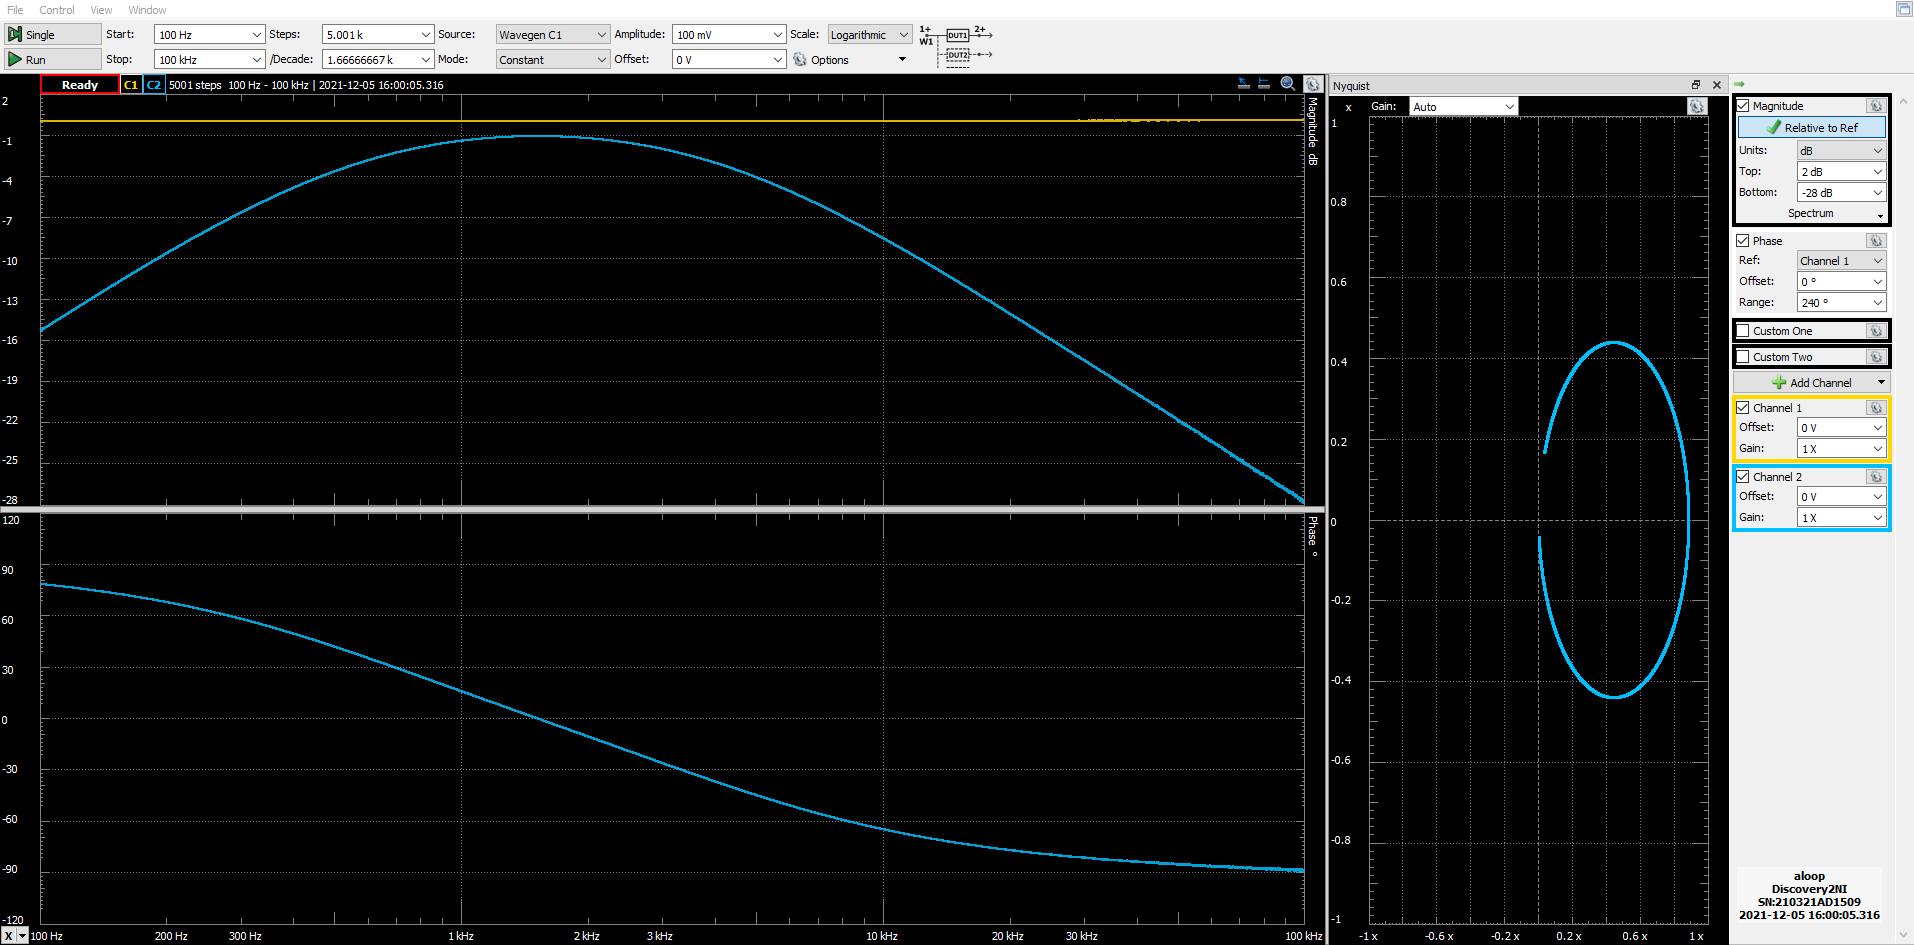
\includegraphics[scale=0.335]{Aloop100Hz}
    \caption{Plot di Bode e Nyquist ottenuto dallo scan con Network tra
    $\SI{100}{\Hz}$ e $\SI{100}{k\Hz}$ con un segnale sinusoidale in ingresso
    all'anello di feedback invertente $A$, di ampiezza costante
    $v\ped{in} = \SI{100}{m\V}$. \label{fig: loopbode}}
\end{figure}

Si è misurata direttamente la frequenza propria dell'oscillatore posizionando
i cursori nel punto in cui la fase si annulla, che corrisponde anche alla
frequenza di centro banda, dove il guadagno della rete di sfasamento è massimo
\begin{align*}
f_0 &= 1522 \pm 2 \; \si{\Hz} \\
A_M &= \abs{\beta(j \omega_0) \bar{A}} =
-1.10 \pm 0.05 \; \si{dB} = 0.881 \pm 0.005
\end{align*}

Dunque abbiamo ricavato una stima delle frequenze di taglio dal punto in cui
il guadagno diminuisce di $-3.01 \; \si{dB}$ rispetto ad $A_M$
\begin{align*}
f_L &= 804 \pm 2 \; \si{\Hz} \\
f_H &= 2875 \pm 8 \; \si{\Hz}
\end{align*}

\subsection{Dipendenza del loop-gain dalla resistenza del potenziometro}
Riportiamo le misure di massimo e minimo guadagno $A_v = V\ped{out}/V_s$
trovate al variare della posizione del trimmer:
\begin{align*}
V_s &= 199 \pm 2 \; \si{m\V} \\
V\ped{min} &= 133.0 \pm 1.1 \; \si{m\V} \implies  A\ped{v, min} =
0.668 \pm 0.009\\
V\ped{max} &= 260 \pm 2 \; \si{m\V} \implies  A\ped{v, max} =
1.306 \pm 0.016\\
\end{align*}

\subsubsection{Misure di guadagno al variare di $V_s$}
Misurando con l'oscilloscopio l'ampiezza dei segnali in ingresso $v\ped{in}$
e in uscita $v\ped{out}$ dall'amplificatore possiamo ricavare una misura del
guadagno del circuito dal rapporto $A = \dfrac{v\ped{out}}{v\ped{in}}$.
\begin{table}[htbp]
\centering
\begin{tabular}{cccc}
\toprule
$v\ped{in}(\si{m\V})$ (nom.) & $v\ped{in} \pm \sigma(v\ped{in})$ [mV] & $v\ped{out} \pm \sigma(v\ped{out})$ [V] & $A \pm \sigma(A)$ \\
\midrule
\midrule
50 & $50.0 \pm 0.4$ & $256 \pm 2 \; \si{m}$ & $5.12 \pm 0.06$ \\
100 & $100.0 \pm 0.8$ & $511 \pm 4 \; \si{m}$ & $5.11 \pm 0.06$ \\
150 & $150.0 \pm 1.2$ & $767 \pm 6$ & $5.11 \pm 0.06$ \\
200 & $200 \pm 1.6$ & $1022 \pm 8$ & $5.11 \pm 0.06$ \\
250 & $250 \pm 2$ & $1278 \pm 11$ & $5.11 \pm 0.06$ \\
300 & $300 \pm 2$ & $1534 \pm 12$ & $5.11 \pm 0.05$ \\
350 & $349 \pm 3$ & $1790 \pm 14$ & $5.13 \pm 0.06$ \\
400 & $399 \pm 3$ & $2046 \pm 16$ & $5.13 \pm 0.06$ \\
450 & $449 \pm 4$ & $2302 \pm 18$ & $5.13 \pm 0.06$ \\
500 & $499 \pm 4$ & $2.56 \pm 0.02$ & $5.13 \pm 0.06$ \\
550 & $549 \pm 4$ & $2.82 \pm 0.02$ & $5.13 \pm 0.06$ \\
600 & $599 \pm 5$ & $3.07 \pm 0.02$ & $5.13 \pm 0.06$ \\
\\
700 & $699 \pm 6$ & $3.55 \pm 0.03$ & $5.07 \pm 0.06$ \\
800 & $799 \pm 6$ & $3.82 \pm 0.03$ & $4.78 \pm 0.05$ \\
900 & $899 \pm 7$ & $3.86 \pm 0.03$ & $4.28 \pm 0.05$ \\
1 V & $999 \pm 8$ & $3.86 \pm 0.03$ & $3.86 \pm 0.04$ \\
1.2 V & $1199 \pm 9$ & $3.86 \pm 0.03$ & $3.22 \pm 0.04$ \\
1.4 V & $1399 \pm 11$ & $3.88 \pm 0.03$ & $2.78 \pm 0.03$ \\
1.6 V & $1599 \pm 12$ & $3.89 \pm 0.03$ & $2.43 \pm 0.03$ \\
1.8 V & $1799 \pm 14$ & $3.90 \pm 0.03$ & $2.17 \pm 0.02$ \\
2 V & $1999 \pm 15$ & $3.92 \pm 0.03$ & $1.96 \pm 0.02$ \\
\bottomrule
\end{tabular} 
\caption{Misure di guadagno al variare della tensione in ingresso
all'amplificatore con $R_2^a = 5.1 \; \si{k\ohm}$. Oltre i \SI{600}{m\V} di
ampiezza del segnale in ingresso la forma d'onda in uscita inizia a
manifestare difetti dovuti al clipping dell'op-amp al di fuori del regime
lineare. \label{tab: gain}}
\end{table}

Con un fit lineare possiamo stimare il guadagno dell'amplificatore a partire
dal grafico di $v\ped{out} = A v\ped{in}$ al variare di $v\ped{in}$.
Riportiamo quanto trovato per il primo circuito:
\begin{figure}[htbp]
\centering
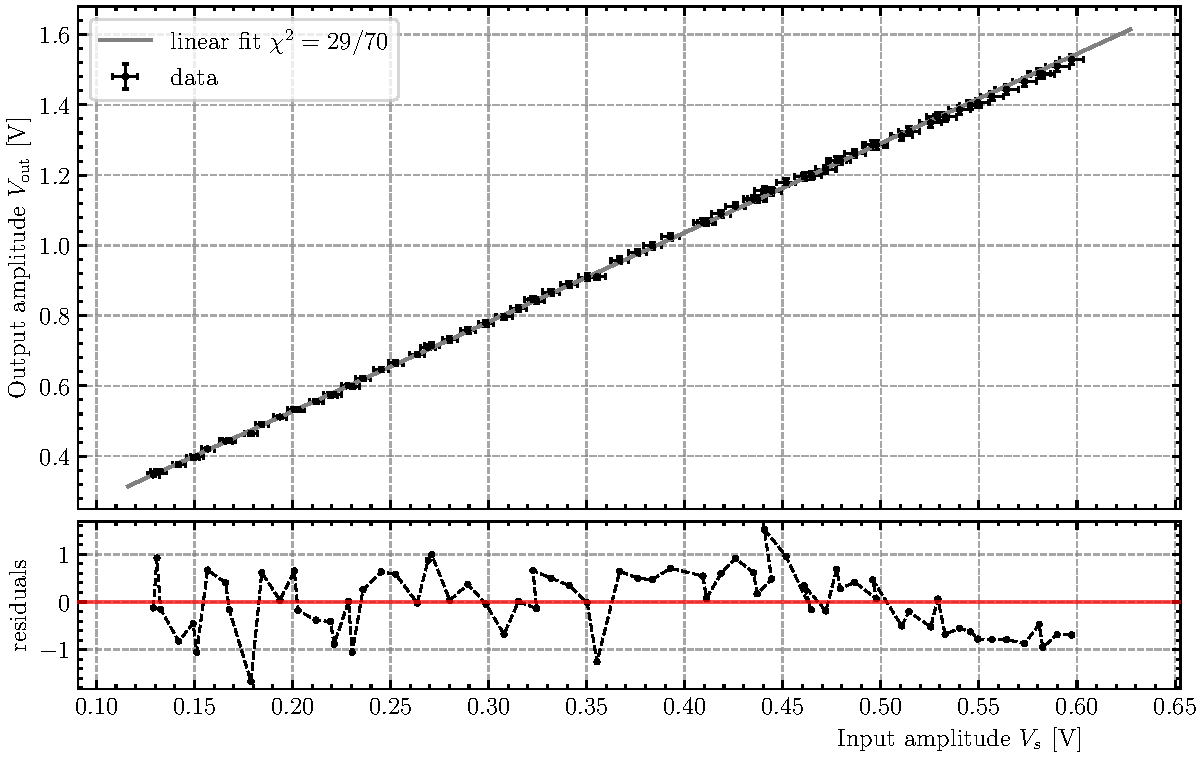
\includegraphics[scale=0.7]{gainfit}
\caption{Fit lineare per l'andamento dell'ampiezza misurata in uscita rispetto
all'ampiezza del segnale in ingresso. \label{fig: gainfit}}
\end{figure}
Da cui troviamo i seguenti parametri per la retta di best-fit
\begin{align*}
\mathrm{intercetta} = -0.6 \pm 0.4 \; \si{m\V} \;\;\;\mathrm{pendenza} = 5.124 \pm 0.003 \;\;\;\mathrm{correlazione} 
= -0.72 \;\;\; \chi^2 = 0.2 \;\;\; d.o.f. = 10 \\
\text{coefficiente angolare/senza intercetta} = 5.120 \pm 0.002 \;\;\;
\chi^2 = 0.2 \;\;\; d.o.f. = 11
\end{align*}

Il valore atteso per il guadagno dal valore dei componenti in questa
configurazione del circuito è pari a
\[
A\ped{v, exp} = -\frac{R_2}{R_1} = - 5.13 \pm 0.12
\]
Questo è in ottimo accordo con quanto trovato sperimentalmente dalla nostra
analisi.

Per completezza riportiamo in un grafico anche le misure che non abbiamo
considerato nel fit perché oltre la regione in cui l'op-amp ha comportamento
lineare
\begin{figure}[htbp]
\centering
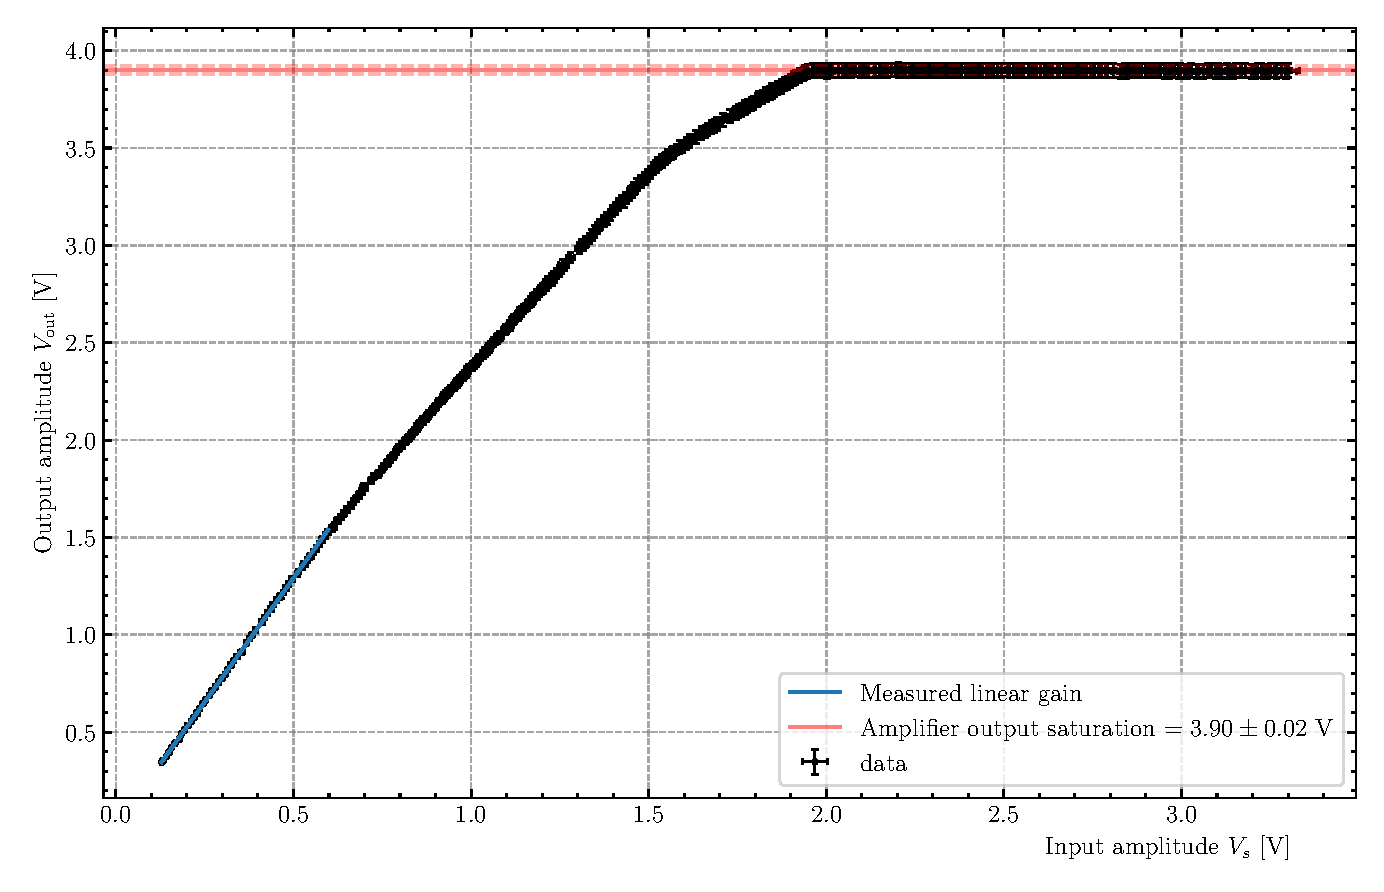
\includegraphics[scale=0.7]{VoutVs}
\caption{Andamento reale dell'ampiezza del segnale in uscita al variare
dell'ampiezza del segnale in ingresso, anche oltre il regime lineare
dell'amplificatore misurati per il circuito con $R_2^a = 5.1 \; \si{k\ohm}$
\label{fig: gainsat}}
\end{figure}

%=======================
\section{Progettazione del circuito auto-oscillante}
Si è completato il circuito oscillatore a ponte di Wien collegando
l'ingresso non-invertente dell'OpAmp TL081CP al punto A, quindi chiudendo
l'anello di feedback positivo, come si vede in \cref{fig: wienschm}
\begin{figure}[htbp]
    \centering
	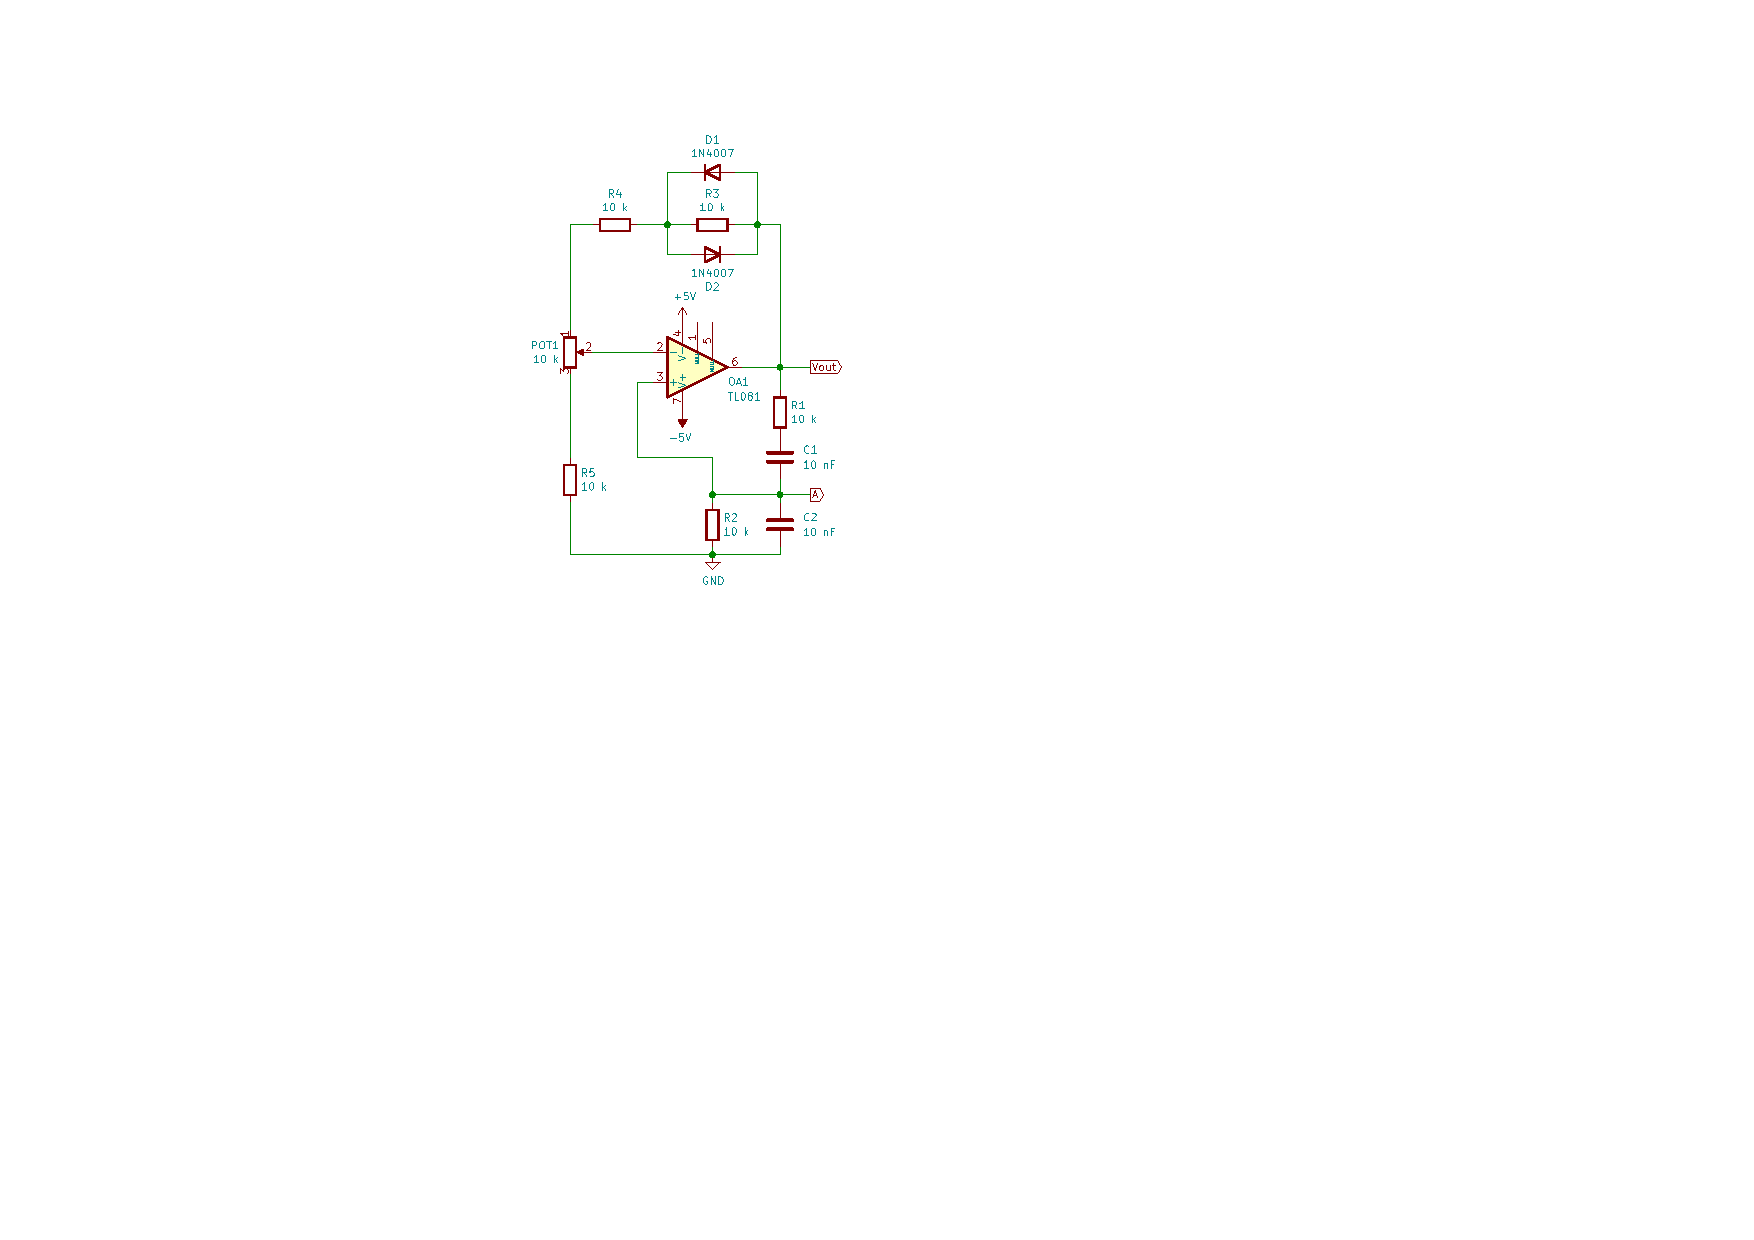
\includegraphics[scale=1.2]{wienschm}
    \caption{Schema circuitale del trigger di Schmitt costruito.
    \label{fig: wienschm}}
\end{figure}

%=======================
\section{Frequenza generata e innesco dell'oscillazione}
Il circuito in \cref{fig: astableschm} è costituito da un trigger di
Schmitt con un filtro passa-basso RC collegato all'ingresso invertente dell'
OpAmp.
\begin{figure}[htbp]
    \centering
%	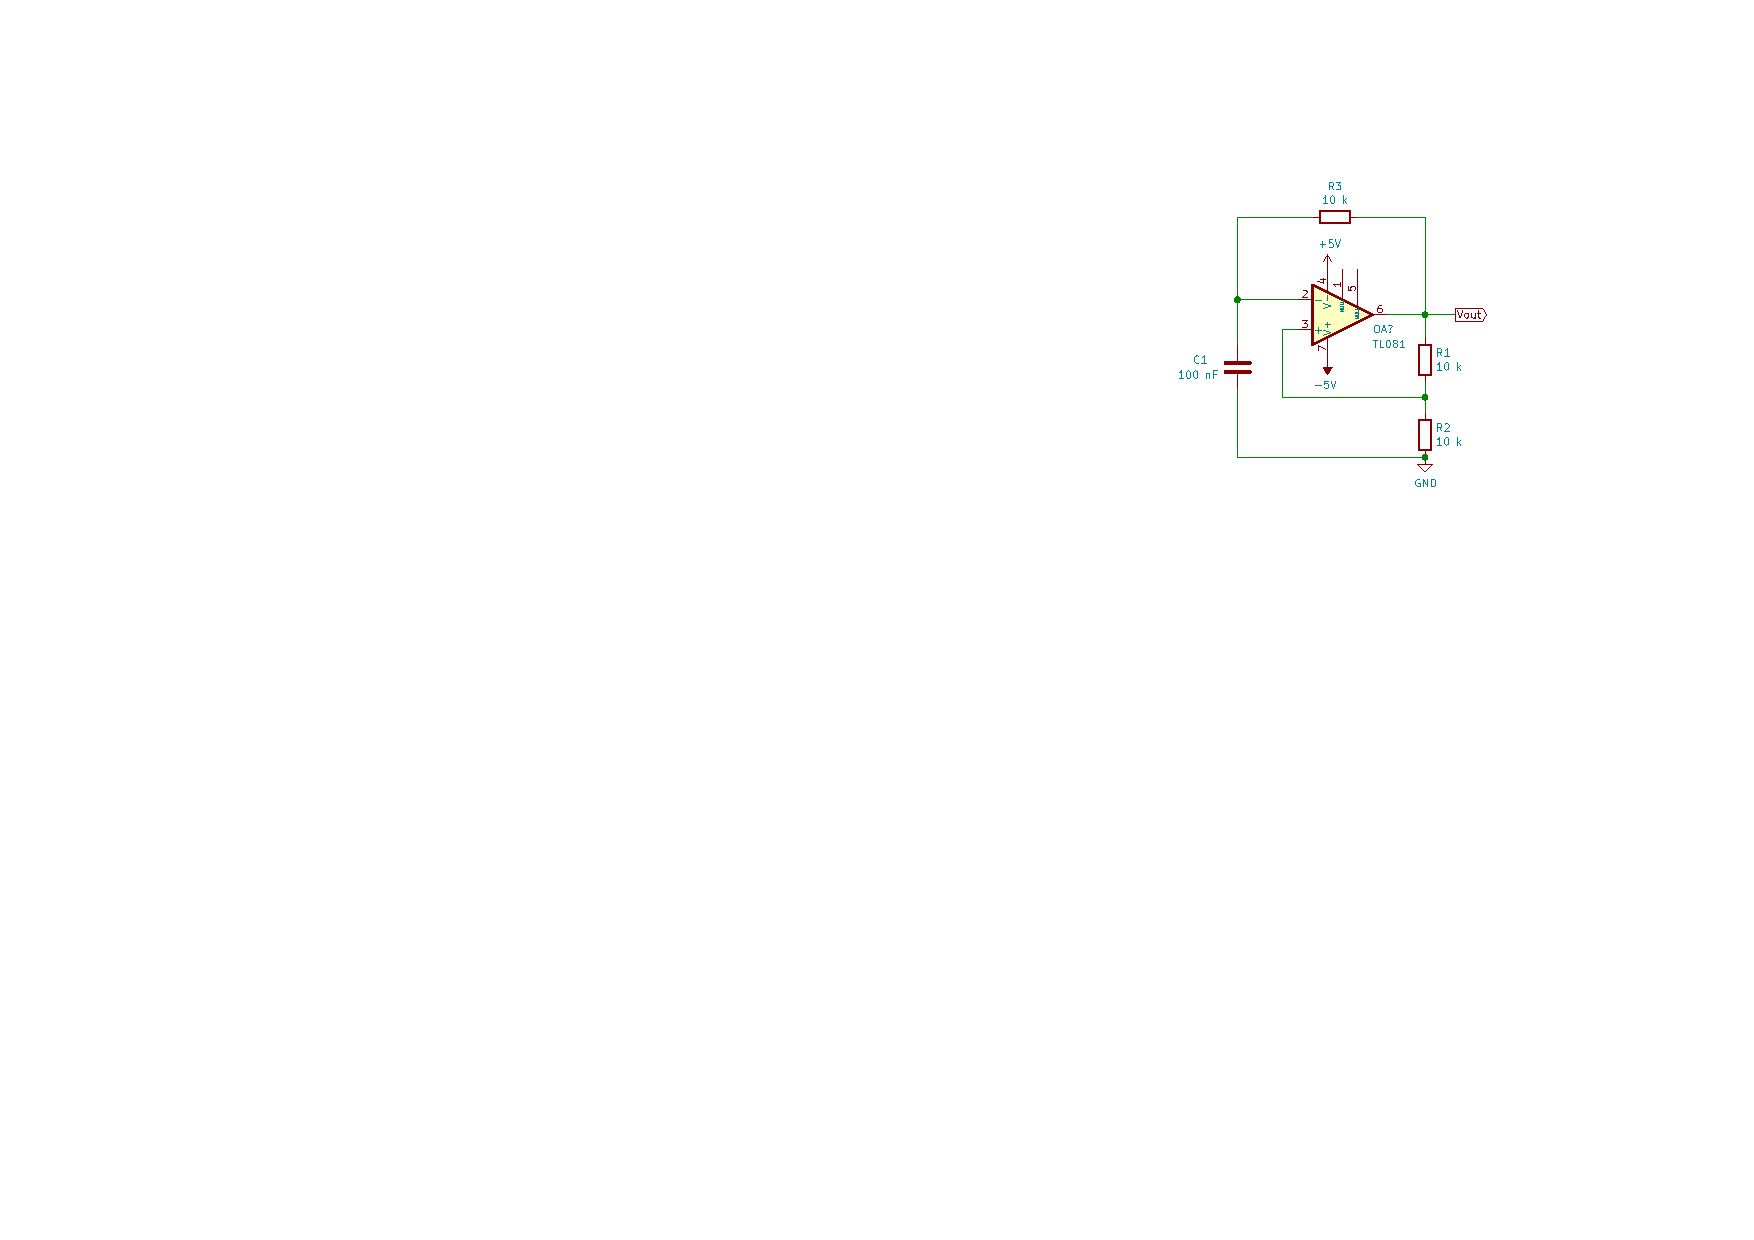
\includegraphics[scale=1.5]{astable}
    \caption{Schema circuitale del multivibratore astabile costruito.
    \label{fig: astableschm}}
\end{figure}

\subsection{Misura della frequenza generata dall'oscillatore}
Per spiegarne il funzionamento è fondamentale studiare il comportamento del
condensatore collegato all'ingresso negativo dell'OpAmp $C_1$. Questo si
carica fino a raggiungere la stessa d.d.p. al terminale positivo
dell'operazionale, a questo punto il trigger cambia rapidamente stato da alto
a basso e, di conseguenza, la tensione all'ingresso non-invertente si abbassa.
Dunque il condensatore comincia a scaricarsi fino a che la d.d.p. ai suoi capi
non raggiunge la stessa tensione ora presente all'ingresso non invertente
dell'amplificatore operazionale.
Il ciclo quindi si ripete generando un'onda quadra in uscita, il cui
periodo di oscillazione è proporzionale al doppio del tempo caratteristico
$\tau = R_3 C_1$ in cui il condensatore è in grado di caricarsi/scaricarsi.

Più precisamente, una volta definite
\begin{align*}
q &= \frac{R_2}{R_1 + R_2} = 0.502 \pm 0.003 \\
\tau &= R_3 C_1 = 95 \pm 4 \; \si{\micro\s}
\end{align*}
Abbiamo come valori attesi per i tempi caratteristici alto $t_H$ e basso
$t_L$ ed il periodo $T$ dell'onda quadra generata dal multivibratore:
\begin{align}
t_H &= \tau \ln\left(\frac{1 - q\frac{V_{OL}}{V_{OH}}}{1-q}\right) =
1.04 \pm 0.04 \; \si{m\s} \\
t_L &= \tau \ln\left(\frac{1 - q\frac{V_{OH}}{V_{OL}}}{1-q}\right) =
1.16 \pm 0.05 \; \si{m\s} \\
\end{align}
Conseguentemente il valore del periodo e duty-cycle atteso valgono:
\begin{align}
T &= t_H + t_L = 2.20 \pm 0.06 \; \si{m\s} \\
\mathrm{dc} &= \frac{t_H}{T} = 47 \pm 2 \; \%
\end{align}

\subsection{Dipendenze dalla posizione del potenziometro}
Osservando il segnale in uscita $V\ped{out} (t)$ ci si aspetta di trovare
un'onda quadra di ampiezza picco-picco $\sim \SI{8}{\V}$, periodo
$T = 2.15 \pm 0.03 \; \si{m\s}$ e duty-cycle $50 \%$. Effettivamente come
tensioni di saturazione alta $V_{OH}$ e bassa $V_{OL}$ dell'onda si è misurato
\begin{align*}
\begin{cases}
V_{OH} &= 4.18 \pm 0.04 \; \si{\V} \\
V_{OL} &= -3.47 \pm 0.03 \; \si{\V}  \implies V\ped{out}^{pp} = 7.65 \pm 0.05
\end{cases}
\end{align*}

Mentre come $v_+ (t)$ ci aspettiamo un'onda della stessa forma di
$V\ped{out} (t)$, ma ridotta in ampiezza di un fattore di partizione
$q \approx 0.5$. Questo corrisponde all'andamento osservato di questi due
segnali, che riportiamo in \cref{fig: v+vout}
\begin{figure}[htbp]
	\centering
%	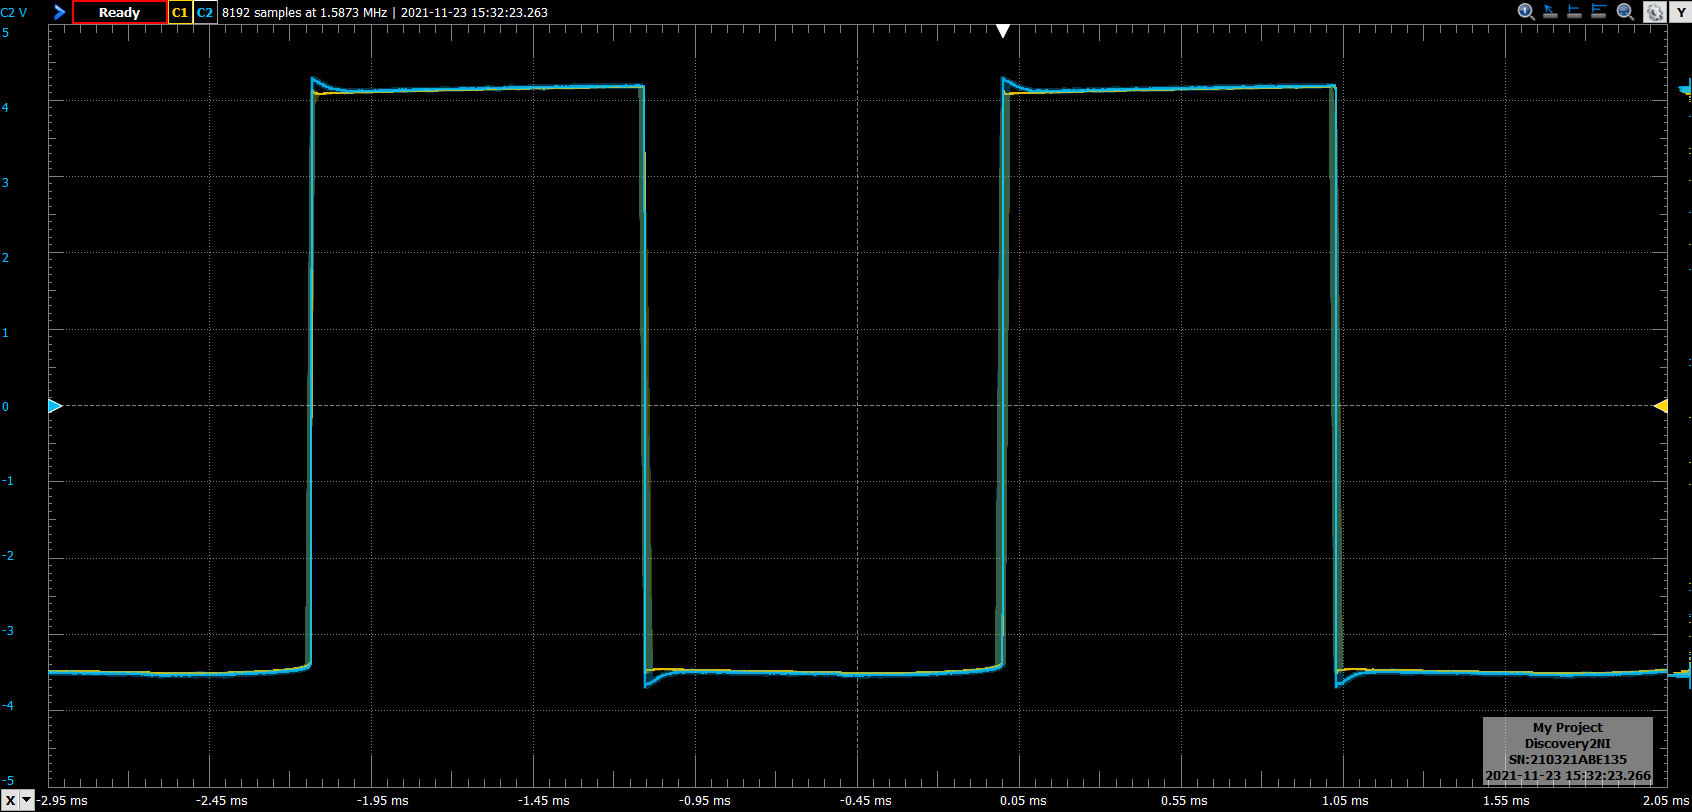
\includegraphics[scale=0.4]{V+Vout}
	\caption{Fermo immagine preso dall'oscilloscopio dell'andamento nel tempo dei
	segnali $v_+ (t)$ (CH1) e $V\ped{out} (t)$ (CH2). \label{fig: v+vout}}
\end{figure}

Osservando $v_- (t)$, infine, ci si aspetta di vedere un segnale ``a pinna di
squalo'', caratteristico del processo di carica/scarica del condensatore e
con la stessa ampiezza di $v_+ (t)$, data dalle tensioni di transizione per
il comparatore/trigger di Schmitt, come riportato in \cref{fig: v-vout}.
\begin{figure}[htbp]
	\centering
%	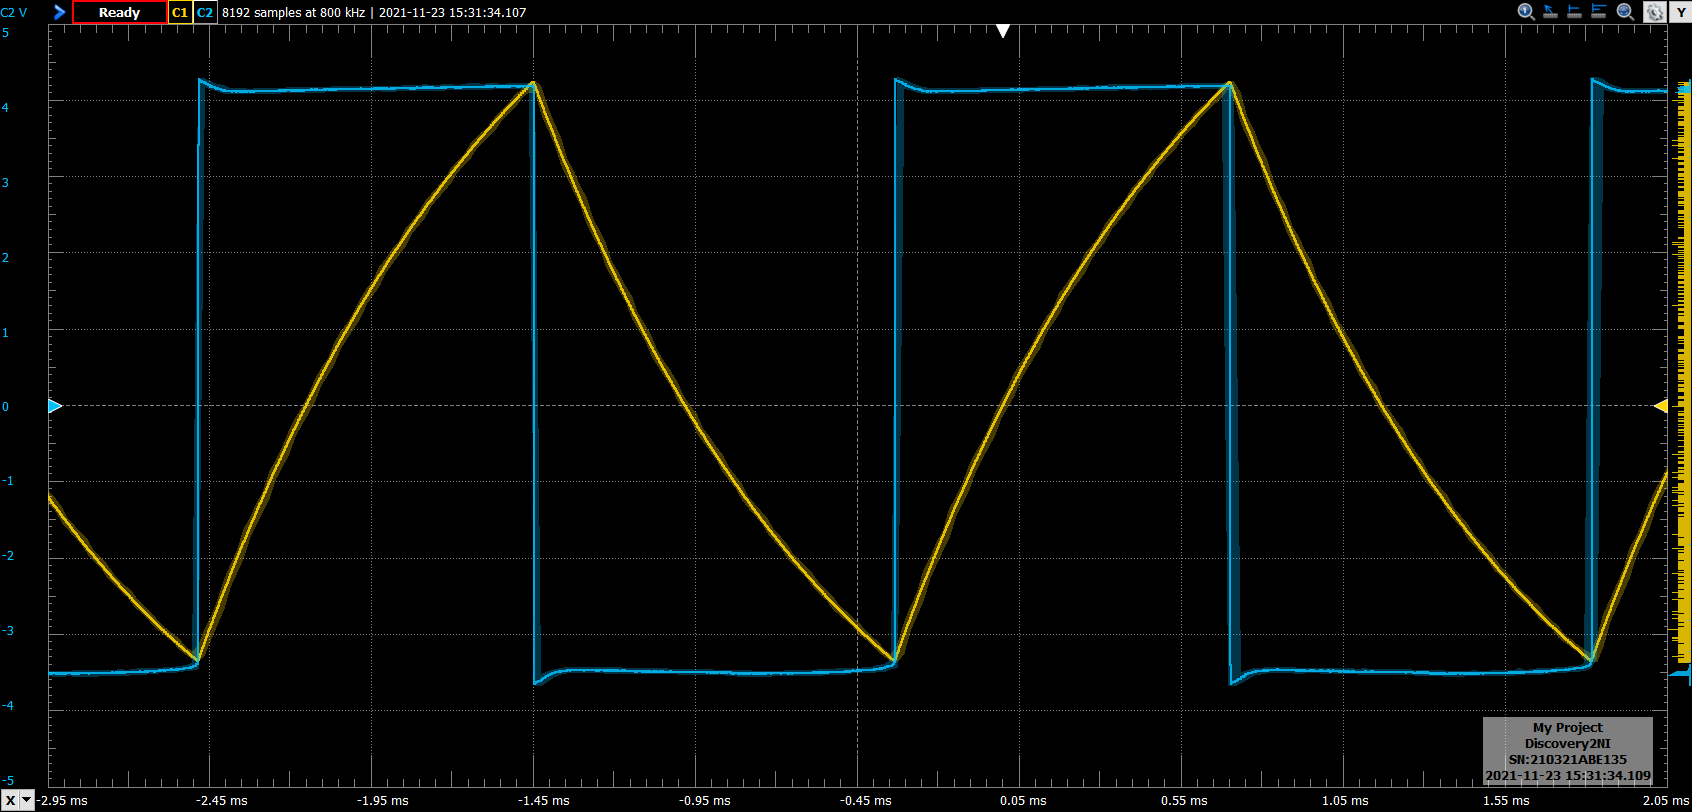
\includegraphics[scale=0.4]{V-Vout}
	\caption{Fermo immagine preso dall'oscilloscopio dell'andamento nel tempo dei
	segnali $v_- (t)$ (CH1) e $V\ped{out}$ (CH2). \label{fig: v-vout}}
\end{figure}

\subsection{Innesco dell'auto-oscillazione}
Per misurare il periodo dell'onda quadra $V\ped{out} (t)$ e la durata dei
tempi in cui è in saturazione positiva $t_H$ (e negativa $t_L$) si è fatto
uso dei cursori sull'asse X:
\begin{align*}
t_H &= 1.03 \pm 0.02 \; \si{m\s} &\quad t_H &= 1.00 \pm 0.02 \; \si{m\s} \\
t_L &= 1.12 \pm 0.02 \; \si{m\s} &\quad t_L &= 1.08 \pm 0.02 \; \si{m\s} \\
T &= 2.14 \pm 0.01 \; \si{m\s}  &\quad T &= 2.09 \pm 0.16 \; \si{m\s} \\
\end{align*}
Da queste abbiamo ricavato la nostra miglior stima del duty-cycle dell'onda
quadra generata dal multivibratore
\begin{align*}
\mathrm{dc} = \frac{t_H}{T} = 47.9 \pm 1.0 \; \% \\
\mathrm{dc} = \frac{t_H}{T} = 48.2 \pm 0.9 \; \% \\
\end{align*}
Le misure dei tempi in saturazione positiva, negativa e del periodo dei
segnali studiati risultano compatibili con i loro valori attesi, per cui
lo è anche il duty cycle.

\subsection{Limite massimo in frequenza del generatore}
Secondo il nostro modello il periodo dell'onda quadra generata è direttamente
proporzionale a (e anche dello stesso ordine di) $\tau = R_3 C_1$, per cui
se ne vogliamo aumentare la frequenza sarà sufficiente ridurre il valore
della resistenza $R_3$ o della capacità $C_1$. Effettivamente abbiamo osservato
un aumento di un fattore $10$ nella frequenza del treno d'impulsi generato,
a seguito di una riduzione di $C_1$ ed $R_3$ dello stesso fattore, in accordo
con quanto ci si aspetta di vedere per una decimazione del tempo caratteristico
di carica/scarica $\tau$.

L'aumento della massima frequenza generabile non è però l'unico effetto che
si osserva per via della modifica di $\tau$: l'onda quadra in uscita risulta
distorta, specialmente intorno ai fronti di salita e discesa che sono
visibilmente limitati in pendenza, come si vede in \cref{fig: astable1nF}.
\begin{figure}[htbp]
	\centering
%	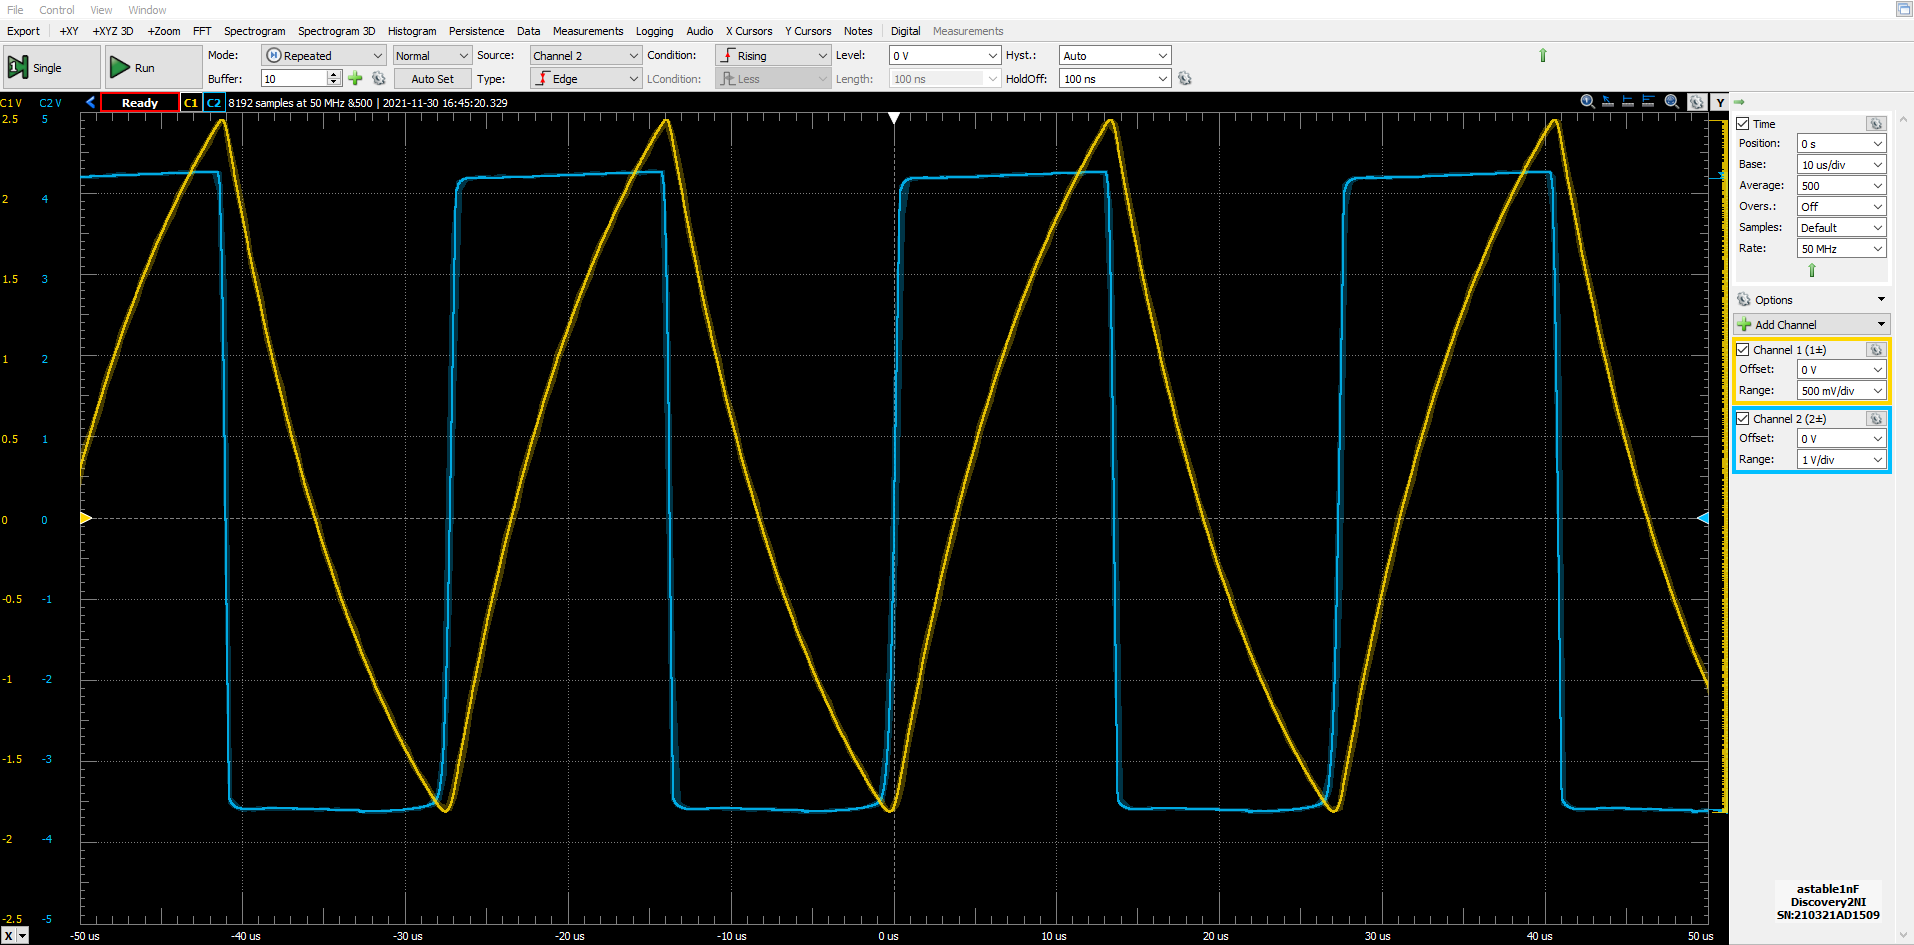
\includegraphics[scale=0.335]{astable1nF}
	\caption{Fermo immagine preso dall'oscilloscopio dell'andamento nel tempo dei
	segnali $v_- (t)$ (CH1) e $V\ped{out} (t)$ (CH2) quando il periodo dell'onda
	generata $T \sim \tau \approx 36 \; \si{\micro\s}$ è ridotto di un fattore di
	circa 10 rispetto alla configurazione originale del circuito.
	\label{fig: astable1nF}}
\end{figure}

In piena analogia con quanto visto nella \cref{sub: trglim}, quando il
semi-periodo dell'uscita si avvicina all'ordine dei $\si{\micro\s}$, cioè il
tempo minimo che l'OpAmp reale impiega per le transizioni di stato dell'onda
quadra di ampiezza picco-picco $V\ped{out}^{pp} \sim \SI{8}{\V}$, il segnale
in uscita presenta fronti di salita e discesa limitati dallo slew-rate
dell'OpAmp, che non riesce a passare abbastanza rapidamente da uno stato
all'altro.

Per verificare che l'effetto di distorsione predominante sia dovuto allo
slew-rate dell'OpAmp, come per il trigger di Schmitt abbiamo misurato (con
i cursori) dalla pendenza dei fronti di salita dell'onda in uscita
$\mathrm{SR} = 11.2 \pm 0.3 \si{V/s}$. Questo è compatibile con l'intervallo
di valori tipici riportato nel datasheet
($\rm SR_{min} = \SI{8}{\V/\micro\s} - SR_{typ} = 13 \; \si{\V/\micro\s}$)
in particolare ci aspettiamo che l'onda quadra generata inizi ad essere
distorta per valori del periodo dell'onda prossimi a
$T\ped{min} \approx 1.4 \; \si{\micro\s}$, compatibilmente con quanto abbiamo
osservato.

Riducendo ulteriormente i valori di resistenza e capacità
($R_3 \approx 220 \; \si{\ohm}$, $C_1 \approx 1 \; \si{nF}$) si osservano
deviazioni ancora più pronunciate dall'onda quadra attesa in uscita, che
possono essere dovute al fatto che il TL081 ha guadagno finito e dipendente
dalla frequenza di lavoro, a differenza di quanto presuppone il nostro modello. 
\begin{figure}[htbp]
	\centering
%	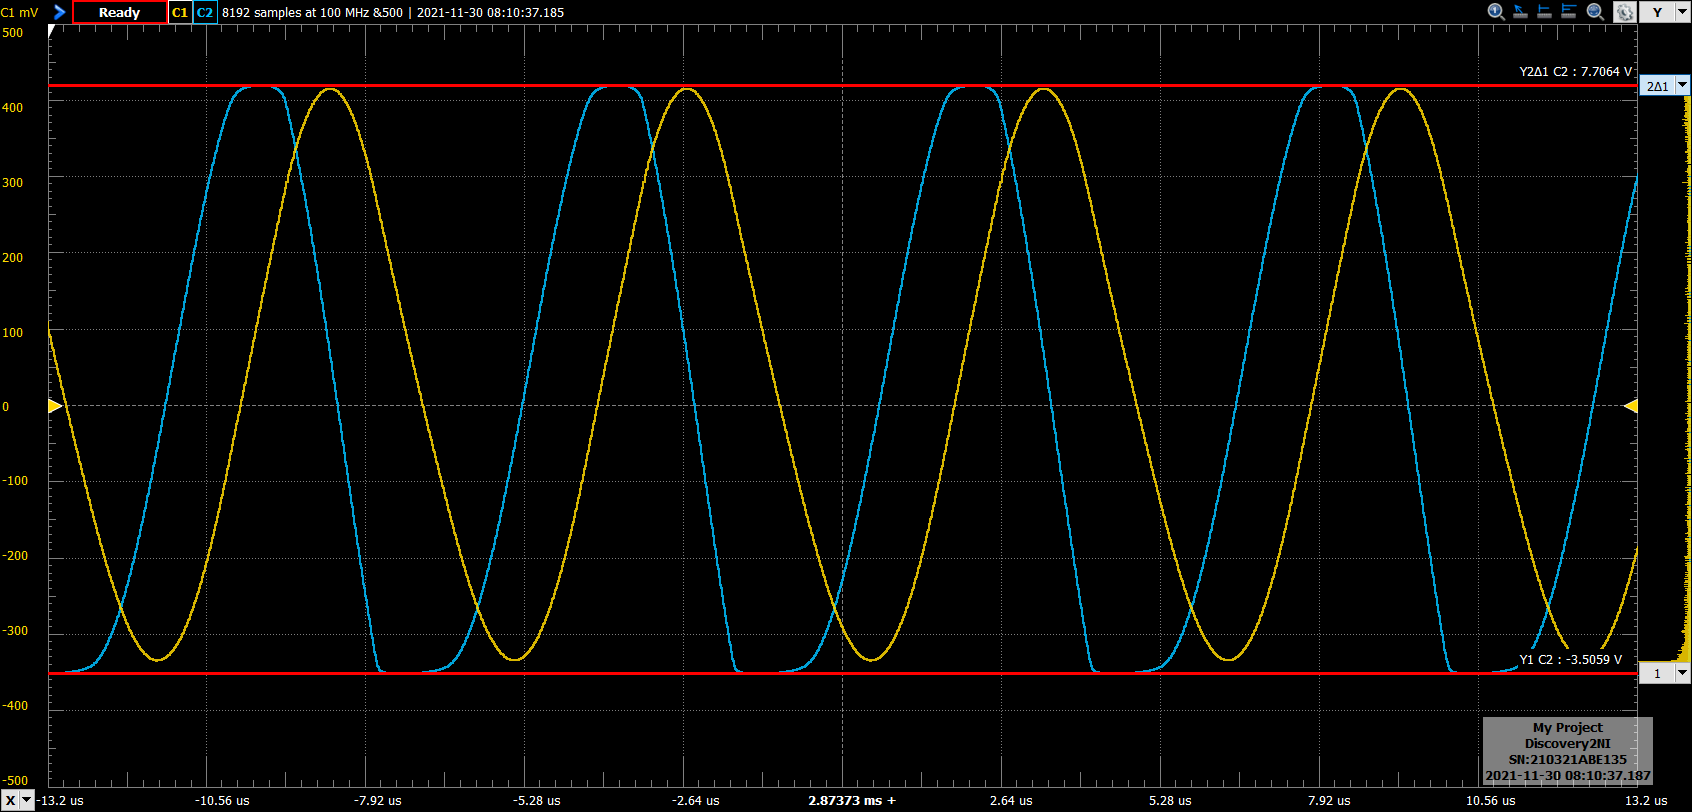
\includegraphics[scale=0.45]{astable(C=1 nF, R= 220 ohm)}
	\caption{Fermo immagine preso dall'oscilloscopio dell'andamento nel tempo dei
	segnali $v_- (t)$ (CH1) e $V\ped{out} (t)$ (CH2) quando il periodo dell'onda
	generata $T \approx \SI{4}{\micro\s}$ è prossimo ai limiti possibili per il
	circuito. \label{fig: astable_lim}}
\end{figure}

%=======================
\section{Funzione dei diodi in parallelo}
Il multivibratore monostabile riportato in \cref{fig: mstableschm} è simile
al circuito precedente, ma ha uno stato stabile (quello alto) e uno instabile,
per cui viene utilizzato come generatore di impulsi. In effetti si è costruito
il circuito a partire dallo stesso trigger di Schmitt invertente, aggiungendo
però un sotto-circuito di trigger all'ingresso positivo dell'OpAmp e il diodo
$D_1$ in parallelo al condensatore $C_1$ del filtro passa-basso.
\begin{figure}[htbp]
    \centering
%	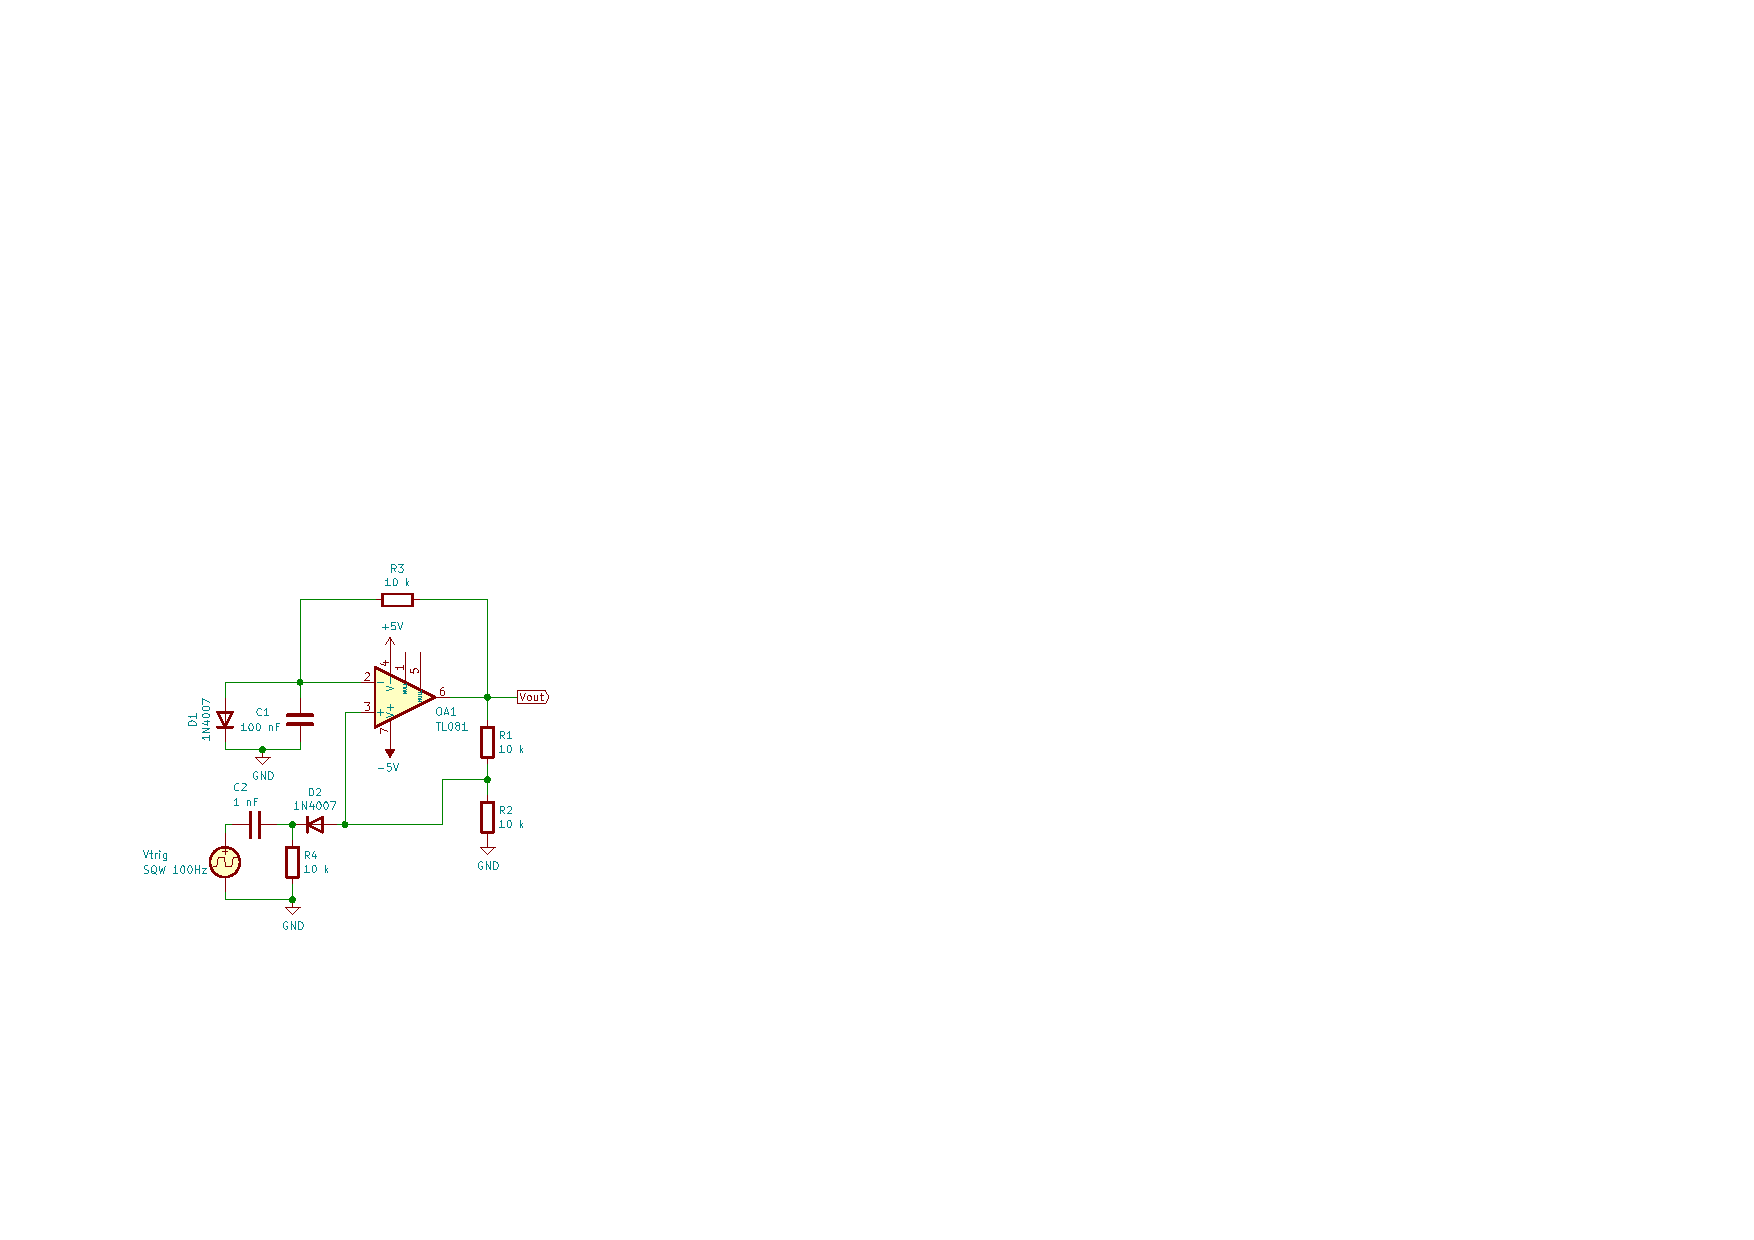
\includegraphics[scale=1.2]{monostable}
    \caption{Schema circuitale del multivibratore monostabile costruito.
    \label{fig: mstableschm}}
\end{figure}

\subsection{Studio dei segnali in ingresso e uscita}
La presenza del diodo in parallelo al condensatore $C_1$ limita la tensione
ai suoi capi $V_C = v_-$, per cui ci aspettiamo di avere
$V_C \leq V\gamma \approx 0.7 \; \si{\V}$, come si trova effettivamente in
\cref{fig: mstabilev-}.
\begin{figure}[htbp]
	\centering
%	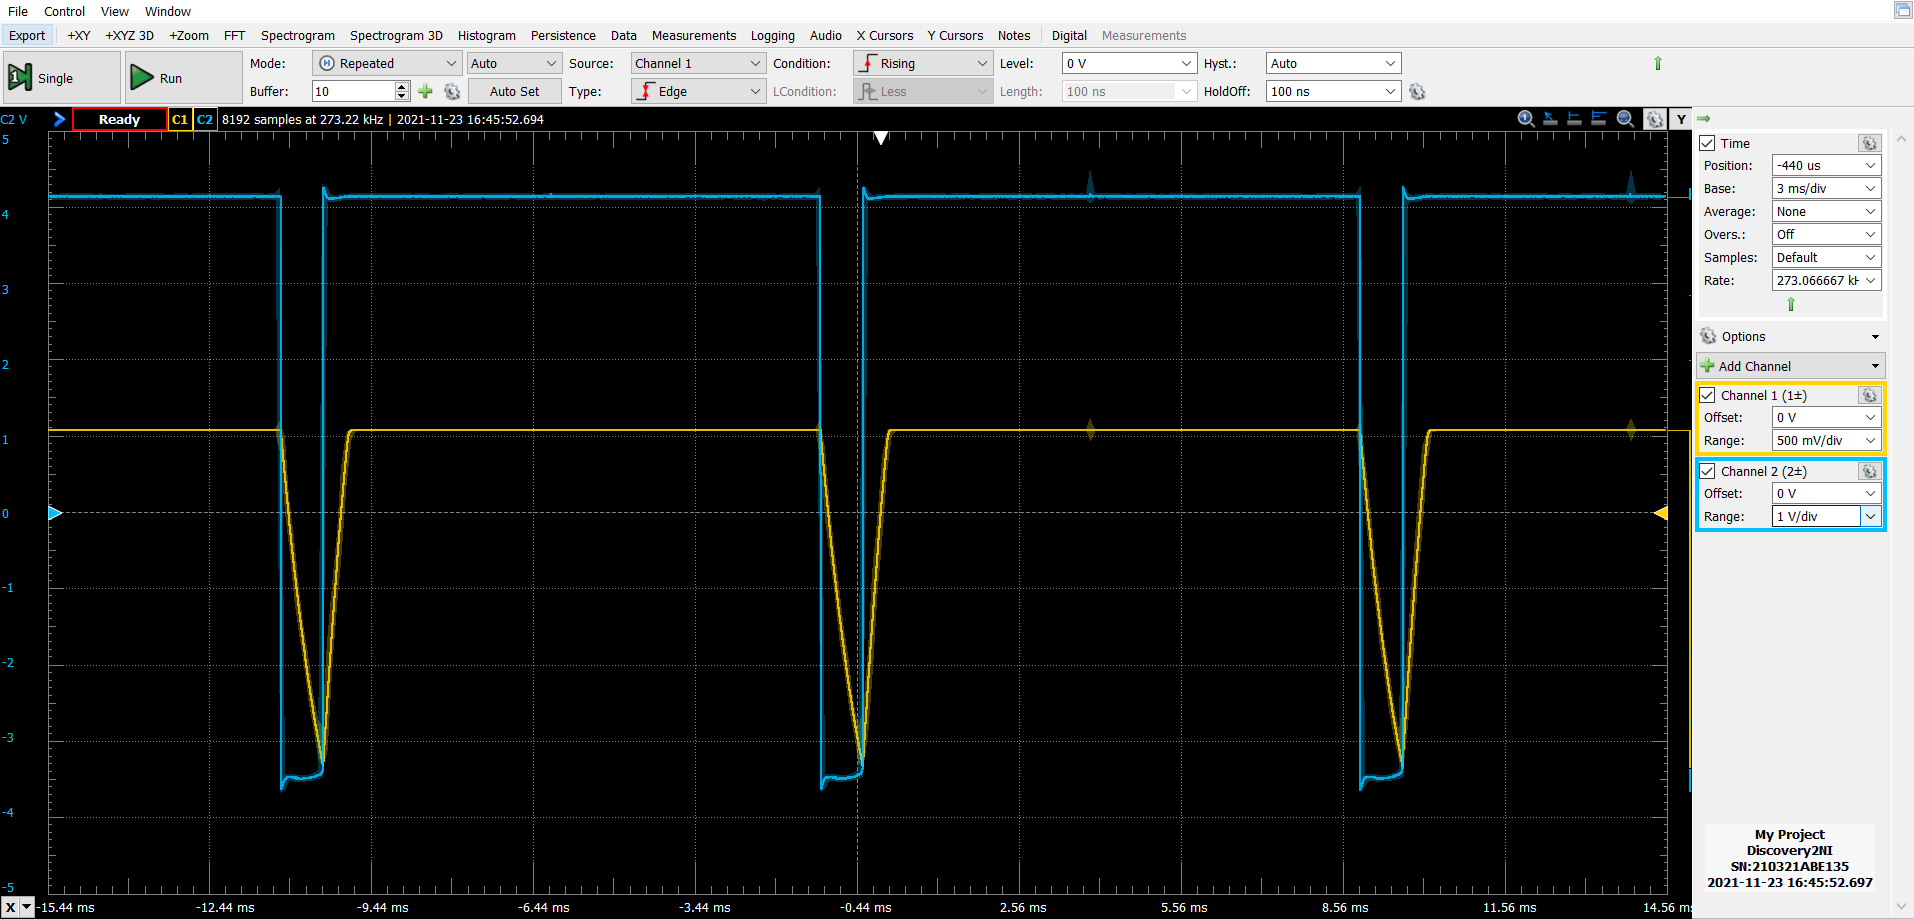
\includegraphics[scale=0.42]{monostabileV-}
	\caption{Acquisizione all'oscilloscopio dell'andamento nel tempo dei
	segnali $v_- (t)$ (CH1) e $V\ped{out} (t)$ (CH2). \label{fig: mstabilev-}}
\end{figure}

\`E per questo che lo stato con l'uscita a livello alto è stabile,
cioè da quest'ultimo il sistema non passa spontaneamente allo stato instabile;
quello con uscita a livello basso.
Dunque per innescare la transizione di stato
$V\ped{out} = V_{OH} \mapsto V_{OL}$ è necessario un circuito di trigger,
che faccia abbassare $v_+$ al di sotto di $v_- \sim V_\gamma$.

In assenza di $V\ped{trig}$, come per il multivibratore astabile, all'ingresso
non-invertente dell'OpAmp ci aspettiamo di trovare come segnale $v_+ (t)$ la
stessa forma d'onda presente all'uscita, ma ridotta in ampiezza di un fattore di partizione $q = \dfrac{R_2}{R_2 + R_1} \approx 0.5$.
Ora però a questa si sovrappongono i picchi di differenza di potenziale che
portano il circuito nello stato instabile sopra descritto; dopo un tempo
caratteristico (proporzionale a $\tau = R_3 C_1$) il multivibratore torna
nella configurazione stabile, generando così un treno di impulsi
negativi/un'onda quadra con duty-cycle prossimo a uno.
Questo è in linea con quanto si vede in \cref{fig: mstabilev+}.
\begin{figure}[htbp]
	\centering
%	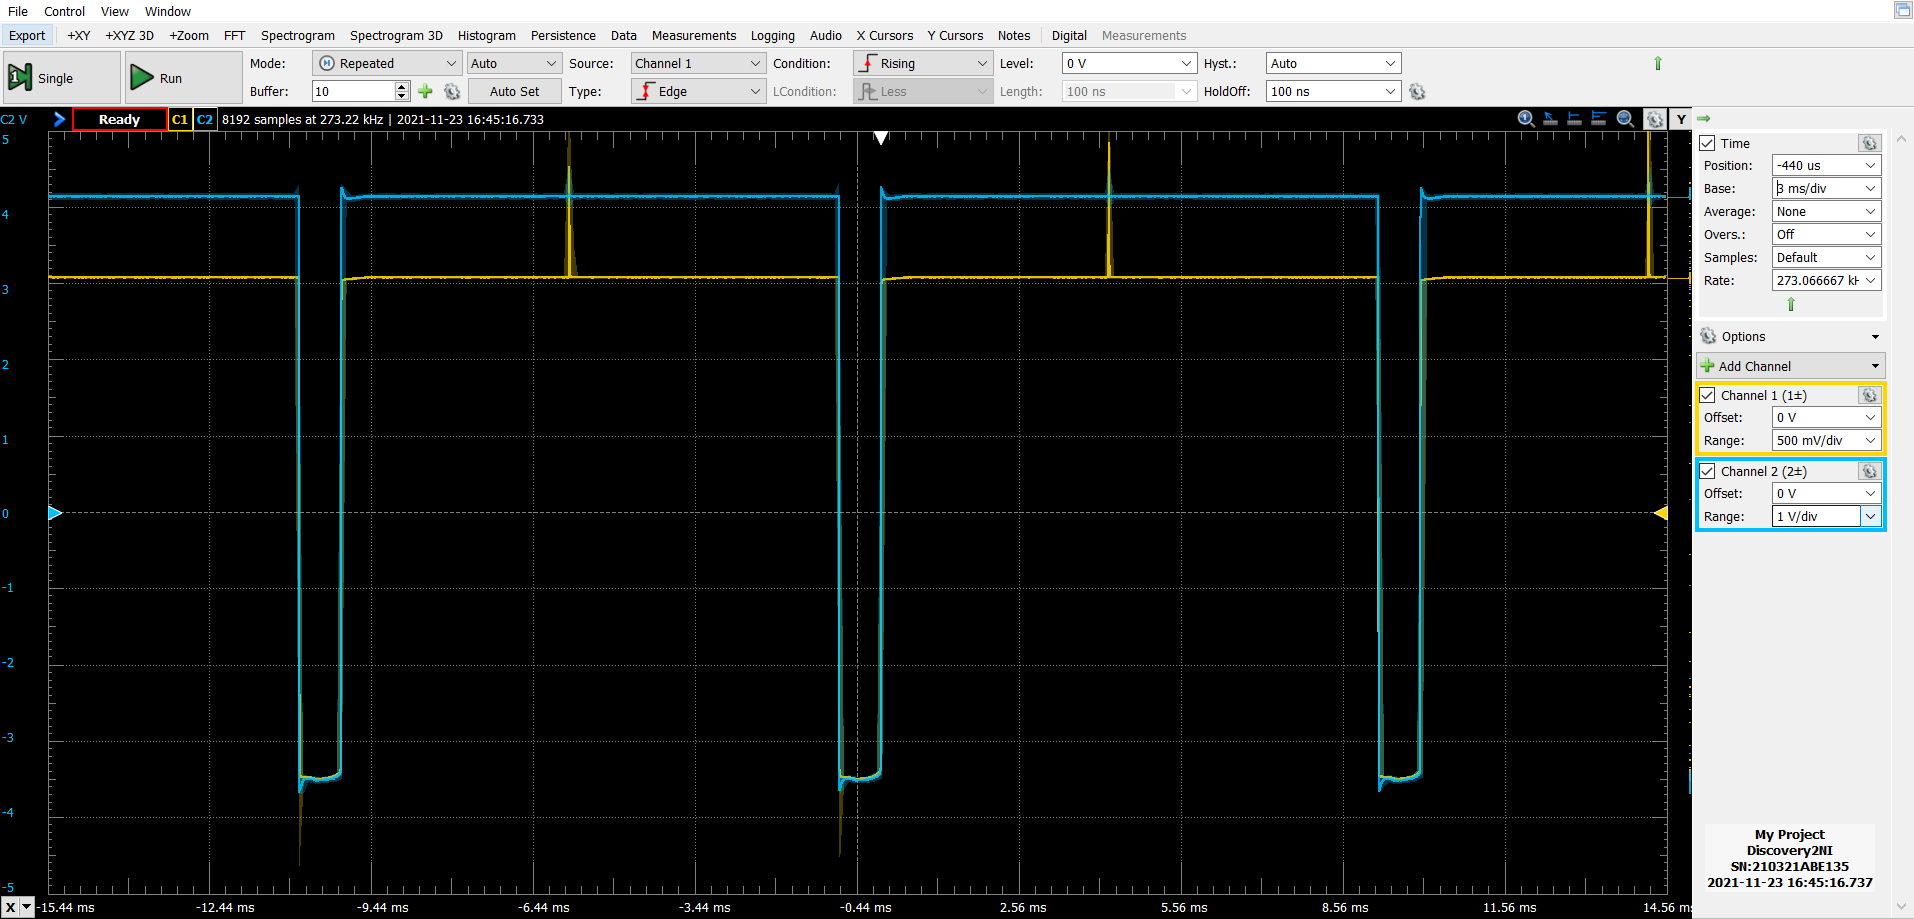
\includegraphics[scale=0.42]{monostabileV+}
	\caption{Acquisizione all'oscilloscopio dell'andamento nel tempo dei
	segnali $v_+ (t)$ (CH1) e $V\ped{out} (t)$ (CH2). \label{fig: mstabilev+}}
\end{figure}

\subsection{Durata dell'impulso generato}
Si è inviata all'ingresso del circuito di trigger un'onda quadra di ampiezza
$V\ped{trig} = 1.99 \pm 0.02 \; \si{\V}$ e frequenza $100 \pm 1.6 \; \si{\Hz}$.

Dunque abbiamo misurato coi cursori le tensioni di saturazione dell'uscita e 
$V_\gamma$ dal livello di tensione costante a cui si trova $v_-$ quando il
circuito è nello stato stabile:
\begin{align*}
V_{OH} &= 4.12 \pm 0.04 \; \si{\V} \quad &V_{OH} &= 4.14 \pm 0.04 \; \si{\V} \\
V_{OL} &= -3.56 \pm 0.03 \; \si{\V} \quad &V_{OL} &= -3.49 \pm 0.03 \; \si{\V} \\
V_{\gamma} &= 547 \pm 6 \; \si{m\V} \quad &V_{\gamma} &= 549 \pm 6 \; \si{m\V}
\end{align*}

E sempre con i cursori si sono misurati i tempi per cui il segnale $V\ped{out}$
rimane ``basso'' in ciascun circuito:
\begin{align*}
t_L &= 767 \pm 10 \;\si{\micro\s} \\
t_L &= 784 \pm 10 \;\si{\micro\s}
\implies \mathrm{dc} = 1 - \frac{t_L}{T} = 92.2 \pm 1.5 \% 
\end{align*}

Il valore atteso per la durata dell'impulso nello stato instabile è legato
al tempo caratteristico in cui si scarica il condensatore $C_1$ dalla
\begin{equation}\label{eq: mstable_Delta}
t\ped{L, exp} = \tau \ln{\left(\frac{1 - V_\gamma/V_{OL}}{1 - q}\right)} =
0.80 \pm 0.03 \; \si{\micro\s}
\end{equation}
Questo risulta compatibile entro l'incertezza con la durata dell'impulso
misurata in uscita dal multivibratore.

\subsection{Analisi del funzionamento del circuito}
Se il condensatore $C_1$ è inizialmente scarico e $V\ped{out} = V_{OH}$, allora
il condensatore in parallelo a $D_1$ si carica fino a quando la d.d.p. tra le
sue armature $V_C \approx V_{\gamma}$. Quindi, poiché $v_- \approx V_{\gamma}$
e $v_+ = \frac{R_{2}}{R_{1} + R_{2}} V\ped{out} \approx \SI{2}{V}$, l'uscita
rimane a livello ``alto''.

Se il condensatore è inizialmente carico (con tensione massima
$v_- \leq V_\gamma$) e se $V\ped{out} = V_{OL}$, allora si scarica fintanto
che vale $v_- \geq v_+ \approx - 1.7 {\V}$. Una volta scarico alla fine
dell'impulso, poiché l'OpAmp è in regime non-lineare, l'uscita commuta
rapidamente (entro i limiti imposti dallo slew-rate) a $V\ped{out} = V_{OH}$;
il condensatore torna a caricarsi e il circuito ritorna alla configurazione
stabile ($v_- \approx V_\gamma$) concludendo il ciclo.

Il sotto-circuito di trigger, formato dal passa-alto $R_4 + C_2$ con il diodo
$D_2$ in cascata, invia all'ingresso non-invertente dell'OpAmp dei picchi di
differenza di potenziale. Questi sono generati grazie al condensatore $C_2$, 
che elimina la componente continua dell'onda quadra $V\ped{trig} (t)$, di cui
ci interessano solamente i fronti ripidi in discesa (e meno in salita).
Infatti è la discesa di $V\ped{trig}$ a generare l'impulso negativo in uscita
dal multivibratore, mentre il fronte di salita è responsabile per i picchi di
tensione positiva che osserviamo in \cref{fig: mstabilev+vtrig}
\begin{figure}[htbp]
	\centering
%	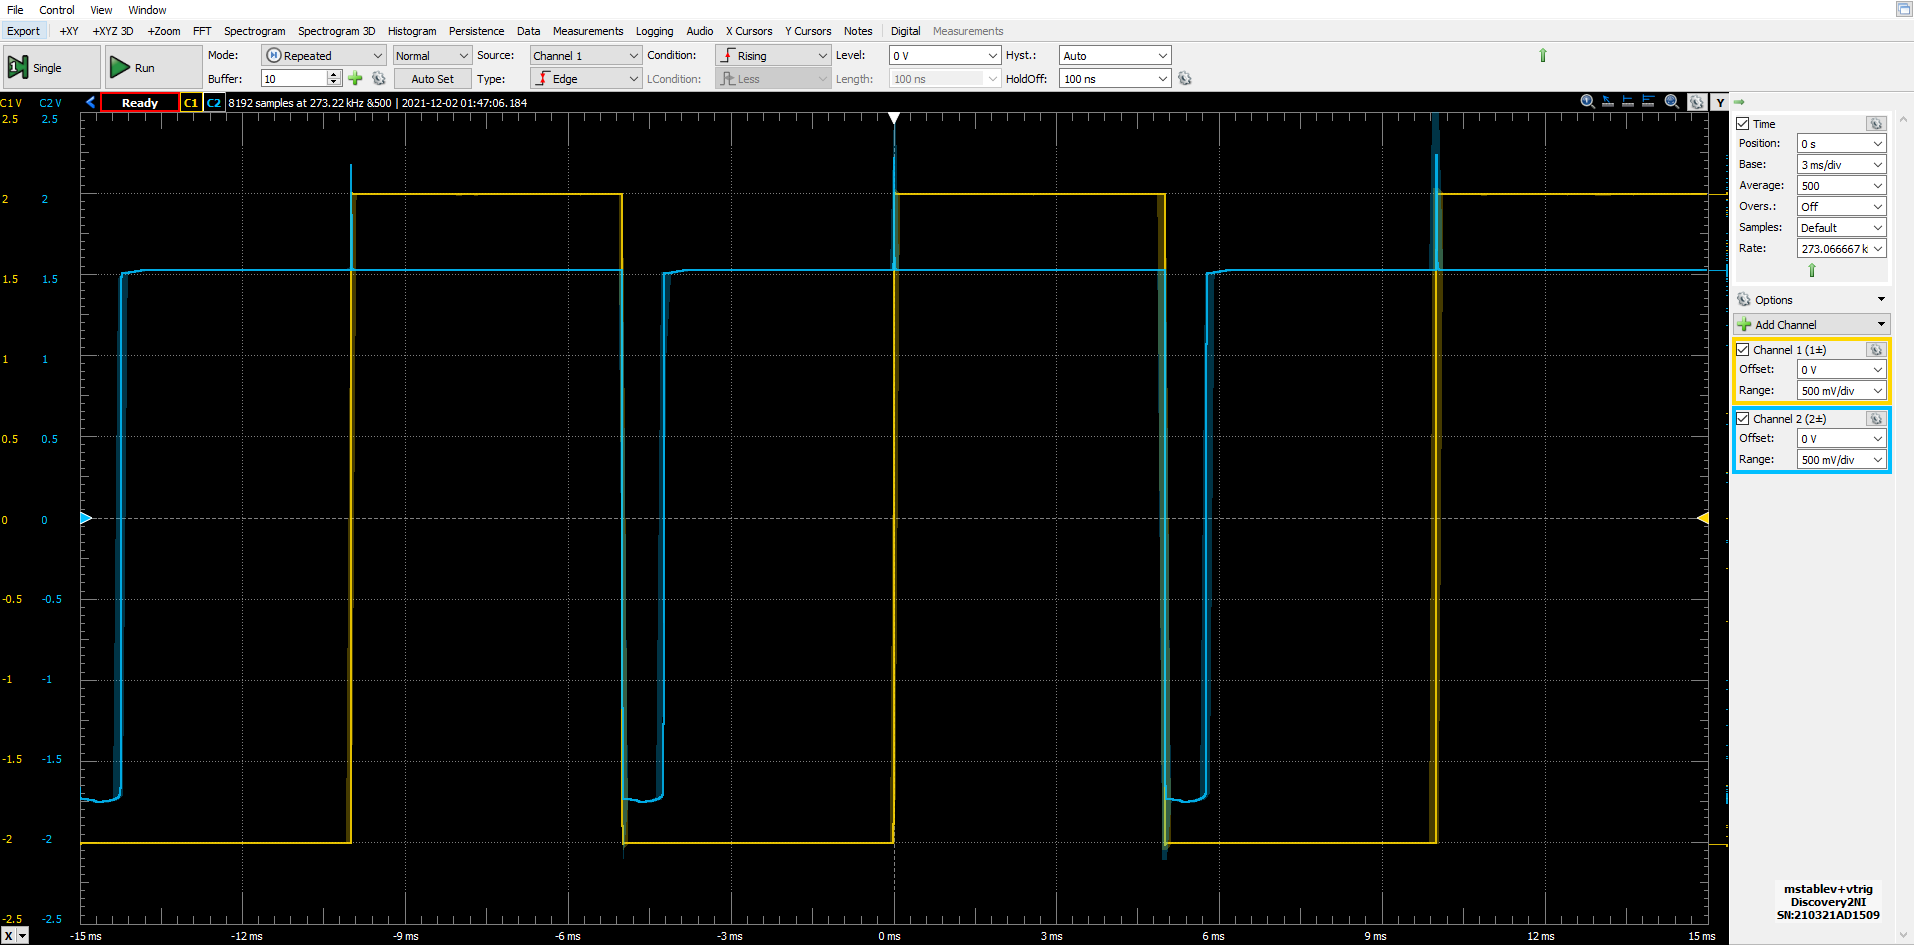
\includegraphics[scale=0.335]{mstablev+vtrig}
	\caption{Acquisizione all'oscilloscopio dell'andamento nel tempo dei
	segnali $V\ped{trig} (t)$ (CH1) e $v_+ (t)$ (CH2).
	\label{fig: mstabilev+vtrig}}
\end{figure}

La risalita del treno d'impulsi in $V\ped{out} (t)$ deve avvenire mentre
$V\ped{trig} (t)$ è ancora costante nel semi-periodo negativo, prima che torni
``alto''. Poiché questa risalita si verifica nel momento in cui $v_- (t)$
assume il suo valore minimo $v_- \approx \frac{1}{2} V_{OL}$ che fa
``scattare'' il comparatore, $C_1$ deve avere il tempo necessario di caricarsi
prima che possa partire una nuova scarica, dunque un nuovo impulso negativo.

Si è quindi tenuta fissa l'ampiezza di $V\ped{trig}$ e se ne è variata la
frequenza. Si osserva che la durata dell'impulso in $V\ped{out}$ rimane
(entro le incertezze di misura) indipendente dalla frequenza del segnale di
trigger, fino a quando la durata dell'impulso è minore del semi-periodo di
$V\ped{trig}$. Al di sopra di questa frequenza critica (sperimentalmente
abbiamo trovato $f\ped{crit} \approx \SI{1}{k\hertz}$) il circuito smette di
funzionare correttamente per durate dell'impulso superiori a
$\frac{1}{2} T\ped{trig} \approx 0.5 \; \si{m\s}$ per via dei tempi di carica
del condensatore $C_1$, come si può vedere in \cref{fig: mstabileflim}.
\begin{figure}[htbp]
	\centering
%	\includegraphics[scale=0.335]{mstable950hz}
	\caption{Acquisizione all'oscilloscopio dell'andamento nel tempo dei
	segnali $v_- (t)$ (CH1) e $V\ped{out} (t)$ (CH2) alla frequenza limite
	per cui è possibile pilotare il multivibratore monostabile.
	\label{fig: mstabileflim}}
\end{figure}

Si è variato il duty-cycle dell'onda $V\ped{trig} (t)$ tenendo fissate
frequenza ed ampiezza. Non abbiamo riscontrato una apprezzabile dipendenza
della durata dell'impulso in $V\ped{out} (t)$ dal duty cycle per il range
esplorato tra l'$1 \%$ e il $99 \%$, come era ragionevole aspettarsi, visto che
utilizziamo solamente i fronti di transizione dell'onda quadra.

Infine abbiamo mantenuto costanti frequenza e duty-cycle di $V\ped{trig} (t)$
e ne abbiamo variato l'ampiezza. La durata dell'impulso in $V\ped{out} (t)$
risulta (entro le incertezze sperimentali) indipendente dall'ampiezza del
segnale di trigger per valori di $V\ped{trig}$ maggiori di una certa soglia.
Si è misurato con i cursori l'ampiezza minima al di sotto della quale
il multivibratore non riesce a compiere la transizione alto-basso,
che risulta
\begin{align*}
V\ped{trig}\ap{min} = 768 \pm 6 \; \si{m\V}
\end{align*}
In effetti, se $V\ped{trig}$ è minore di questa soglia ci aspettiamo
che $v_+ (t)$, quindi gli impulsi prodotti dal trigger sovrapposti al segnale
in uscita dal partitore, non siano abbastanza grandi da rendere
$v_d = v_+ - v_- < \SI{0}{\V}$ e quindi far commutare il discriminatore; perciò
$V\ped{out}$ rimane fisso alla tensione di saturazione alta, che
corrisponde a quanto si è osservato dall'esperimento.

\section{Misure di guadagno dell'oscillatore}

%=======================
\section*{Conclusioni e commenti finali}
Si è riusciti a costruire e studiare alcuni dei circuiti più semplici e noti
che fanno uso di amplificatori operazionali in regime non lineare, tra cui:
un amplificatore di carica, un trigger di Schmitt e due multivibratori; uno
astabile e uno monostabile.

In particolare siamo riusciti a descrivere e verificare sperimentalmente il
funzionamento dei circuiti e a caratterizzarne tempi e frequenze
caratteristici; dunque anche i limiti fisici in frequenza, ampiezza e
duty-cycle sia per i segnali in ingresso che nella risposta all'uscita.

%=======================
\section*{Dichiarazione}
I firmatari di questa relazione dichiarano che il contenuto della relazione \`e
originale, con misure effettuate dai membri del gruppo, e che tutti i firmatari
hanno contribuito alla elaborazione della relazione stessa.
\end{document}
